%\documentclass[compress]{beamer}
\documentclass[8pt]{beamer}

%-----------------------------------------------------------
% PACKAGES

%\usepackage[latin1]{inputenc}
\mode<presentation>

%\usepackage[T1]{fontenc}  
\usetheme{Warsaw}
%\usetheme{Madrid}

\usepackage{graphicx}
%\usepackage[section]{placeins} % force � mettre l'image o� on veut
%\usepackage{float} %utiliser H pour forcer � mettre l'image o� on veut
\usepackage{lscape} %utilisation du mode paysage
%\usepackage{pslatex}
\usepackage{url}
\usepackage{subfigure}
\usepackage{caption}
%\usepackage{subcaption}

\usepackage{graphicx}
\usepackage{tabls}
\usepackage{afterpage}

%\usepackage[]{media9}
\usepackage{multimedia}

\usepackage{amsthm}
\usepackage{amssymb}
\usepackage{amsmath}
\usepackage{amsfonts}
\usepackage{amstext}
\usepackage{amsbsy}
\usepackage{mathbbol} 


\usepackage{epsfig}
%\usepackage{epsfig}
%\usepackage{cites}
\usepackage{epsf}
\usepackage{array}
\usepackage{color}

%-----------------------------------------------------------
% NEW  DEFINITIONS
%
%=================================================================================================
% new commands
% +++++++++++++++++++++++++++++++++++++++++++++++++++++++++++++++++++++++++++++++++++++++++++++++++
\newcommand{\nc}{\newcommand}

% operators
\renewcommand{\div}{\mbold{\nabla}\! \cdot \!}
\newcommand{\grad}{\mbold{\nabla}}
\newcommand{\divv}[1]{\boldsymbol{\nabla}^{#1}\! \cdot \!}
\newcommand{\gradd}[1]{\mbold{\nabla}^{#1}}
\newcommand{\mbold}[1]{\boldsymbol#1}
% latex shortcuts
\newcommand{\bea}{\begin{eqnarray}}
\newcommand{\eea}{\end{eqnarray}}
\newcommand{\be}{\begin{equation}}
\newcommand{\ee}{\end{equation}}
\newcommand{\bal}{\begin{align}}
\newcommand{\eali}{\end{align}}
\newcommand{\bi}{\begin{itemize}}
\newcommand{\ei}{\end{itemize}}
\newcommand{\ben}{\begin{enumerate}}
\newcommand{\een}{\end{enumerate}}
\usepackage{amsthm}
\newtheorem*{remark}{Remark}
% DGFEM commands
\newcommand{\jmp}[1]{[\![#1]\!]}                     % jump
\newcommand{\mvl}[1]{\{\!\!\{#1\}\!\!\}}             % mean value
\newcommand{\keff}{\ensuremath{k_{\textit{eff}}}\xspace}
% shortcut for domain notation
\newcommand{\D}{\mathcal{D}}
% vector shortcuts
\newcommand{\vo}{\mbold{\Omega}}
\newcommand{\vr}{\mbold{r}}
\newcommand{\vn}{\mbold{n}}
\newcommand{\vnk}{\mbold{\mathbf{n}}}
\newcommand{\vj}{\mbold{J}}
\newcommand{\eig}[1]{\| #1 \|_2}
%
\newcommand{\EI}{\mathcal{E}_h^i}
\newcommand{\ED}{\mathcal{E}_h^{\partial \D^d}}
\newcommand{\EN}{\mathcal{E}_h^{\partial \D^n}}
\newcommand{\ER}{\mathcal{E}_h^{\partial \D^r}}
\newcommand{\reg}{\textit{reg}}
%
\newcommand{\norm}{\textrm{norm}}
\renewcommand{\Re}{\textrm{Re}}
\newcommand{\Pe}{\textrm{P\'e}}
\renewcommand{\Pr}{\textrm{Pr}}
%
\newcommand{\resi}{R}
%\newcommand{\resinew}{\tilde{D}_e}
\newcommand{\resinew}{\widetilde{\resi}}
\newcommand{\resisource}{\widetilde{\resi}^{source}}
\newcommand{\matder}[1]{\frac{\textrm{D} #1}{\textrm{D} t}}
%
% extra space
\newcommand{\qq}{\quad\quad}
% common reference commands
\newcommand{\eqt}[1]{Eq.~(\ref{#1})}                     % equation
\newcommand{\fig}[1]{Fig.~\ref{#1}}                      % figure
\newcommand{\tbl}[1]{Table~\ref{#1}}                     % table
\newcommand{\sct}[1]{Section~\ref{#1}}                   % section
\newcommand{\app}[1]{Appendix~\ref{#1}}                   % appendix
%
\newcommand{\ie}{i.e.,\@\xspace}
\newcommand{\eg}{e.g.,\@\xspace}
\newcommand{\psc}[1]{{\sc {#1}}}
\newcommand{\rs}{\psc{R7}\xspace}
%
\newcommand\br{\mathbf{r}}
%\newcommand{\tf}{\varphi}
\newcommand{\tf}{b}
%
\newcommand{\tcr}[1]{\textcolor{red}{#1}}
\newcommand{\tcb}[1]{\textcolor{blue}{#1}}
\newcommand{\mt}[1]{\marginpar{ {\tiny #1}}}

\newcommand{\bs}[1]{\mathbf{#1}}
\renewcommand{\bs}[1]{\vec{#1}}
%\newcommand{\dd}{\mathrm{d}}
\newcommand{\norm}{\textrm{norm}}
\renewcommand{\Re}{\textrm{Re}}
\newcommand{\Pe}{\textrm{P\'e}}
\renewcommand{\Pr}{\textrm{Pr}}

\newcommand{\resi}{R_e}
%\newcommand{\resinew}{\tilde{D}_e}
\newcommand{\resinew}{\widetilde{\resi}}
\newcommand{\matder}[1]{\frac{\textrm{D} #1}{\textrm{D} t}}

\newcommand{\divv}[1]{\vec{\nabla}^{#1}\! \cdot \!}
\newcommand{\gradd}[1]{\vec{\nabla}^{#1}}

\newcommand{\tcr}[1]{\textcolor{red}{#1}}
\newcommand{\tcb}[1]{\textcolor{blue}{#1}}
\newcommand{\tcm}[1]{\textcolor{magenta}{#1}}

%=================================================================================================

%============================================================

%style et couleur
%\usetheme{Frankfurt}
\date{09/09/2015}

%\addtobeamertemplate{footline}{\hfill\insertframenumber/\inserttotalframenumber\hspace{2em}\null}

\setbeamertemplate{footline}{
\leavevmode%
%\hbox{\hspace*{-0.06cm}
\begin{beamercolorbox}[wd=.5\paperwidth,ht=3.25ex,dp=1ex,center]{author in head/foot}%
	\usebeamerfont{author in head/foot}\insertshortauthor%~~(\insertshortinstitute)
\end{beamercolorbox}%
\begin{beamercolorbox}[wd=.25\paperwidth,ht=3.25ex,dp=1ex,center]{section in head/foot}%
	\usebeamerfont{section in head/foot} Multimat 2015, W\"urburg % \insertshorttitle
\end{beamercolorbox}%
\begin{beamercolorbox}[wd=.25\paperwidth,ht=3.25ex,dp=1ex,left]{section in head/foot}%
	\usebeamerfont{section in head/foot}\insertshortdate{}\hspace*{2em}
	\insertframenumber{} / \inserttotalframenumber %\hspace*{2ex}
\end{beamercolorbox}}%
%\vskip0pt%
%}

\beamertemplatetransparentcovered

\urldef{\ragusa}\url{jean.ragusa@tamu.edu}
\urldef{\delchini}\url{delcmo@tamu.edu}
\urldef{\morel}\url{morel@tamu.edu}

\title{Entropy-based artificial viscosity stabilization for non-equilibrium Grey
Radiation-Hydrodynamics}

\author{Marc O. Delchini, \underline{Jean C. Ragusa}, Jim E. Morel}
\institute{{\large  Texas A\&M University, College Station, TX, USA}}

%%%%%%%%%%%%%%%%%%%%%%%%%%%%%%%%%%%%%%%%%%%%%%%%%%%%%%%%%%%%%%%%%%%%

\begin{document}

\begin{frame}
\titlepage
\small{emails:  {\delchini}, {\ragusa}, {\morel} }

\end{frame}

\begin{frame}
	\frametitle{Outline}
	\tableofcontents 
\end{frame}

%%%%%%%%%%%%%%%%%%%%%%%%%%%%%%%%%%%%%%%%%%%%%%%%%%%%%%%%%%%%%%%%%%%%
%%%%%%%%%%%%%%%%%%%%%%%%%%%%%%%%%%%%%%%%%%%%%%%%%%%%%%%%%%%%%%%%%%%%
\section{Background and Motivation}
%%%%%%%%%%%%%%%%%%%%%%%%%%%%%%%%%%%%%%%%%%%%%%%%%%%%%%%%%%%%%%%%%%%%
%%%%%%%%%%%%%%%%%%%%%%%%%%%%%%%%%%%%%%%%%%%%%%%%%%%%%%%%%%%%%%%%%%%%

%%%%%%%%%%%%%%%%%%%%%%%%%%%%%%%%%%%%%%%%%%%%%%%%%%%%%%%%%%%%%%%%%%%%
\subsection{Grey Radiation-Hydrodynamics}
%%%%%%%%%%%%%%%%%%%%%%%%%%%%%%%%%%%%%%%%%%%%%%%%%%%%%%%%%%%%%%%%%%%%



%%%%%%%%%%%%%%%%%%%%%%%%%%%%%%%%%%%%%%%%%%%%%%%%%%%%%%%%%%%%%%%%%%%%
\begin{frame} 
\frametitle{Grey Radiation-Hydrodynamics (GRHD)}

\begin{block}{GRHD system of equations }
\begin{align}
&\partial_t \left( \rho \right) + \partial_x\left( \rho u \right) = 0 \nonumber  \\
%
&\partial_t \left( \rho u\right) + \partial_x \left(\rho u^2 + P  \right) = {\color{blue}-\partial_x \left(\frac{\epsilon}{3}\right)} \nonumber\\
&\partial_t \left( \rho E\right) + \partial_x \left[ u \left( \rho E + P \right) \right] = {\color{blue}-\frac{u}{3} \partial_x \epsilon - \sigma_a c \left( a T^4 - \epsilon \right)} \nonumber  \\
%
&\partial_t \epsilon + \frac{4}{3} \partial_x \left( u \epsilon \right) = {\color{blue}\frac{u}{3} \partial_x \epsilon} + {\color{magenta}\partial_x \left( \frac{c}{3 \sigma_t} \partial_x \epsilon \right)} + {\color{blue}\sigma_a c \left( a T^4 - \epsilon \right)} \nonumber
\nonumber
\end{align}
 $\rho$, $u$, $E$, $\epsilon$, $P$ and $T$ are the material density, material velocity, material specific total energy, radiation energy density, material pressure and temperature, respectively. The total and absorption cross sections, $\sigma_t$ and $\sigma_a$, are either constant or are expressed as a function of material density and temperature. The variables $a$ and $c$ are the radiation constant and the speed of light, respectively.
\end{block}

\begin{block}{A few remarks:}
\begin{itemize}
\setlength{\itemsep}{10pt}
\item Relaxation term in the energy and radiation equations: ${\color{blue}\sigma_a c \left( a T^4 - \epsilon \right)}$.% behaves like a diffusion term when $\sigma_a \to \infty$ \cite{ShiJin}.
\item Diffusion term: ${\color{magenta}\partial_x \left( \frac{c}{3 \sigma_t} \partial_x \epsilon \right)}$.
\item The above system of equations is NOT hyperbolic, and yet ...
\end{itemize}
\end{block}

\end{frame}
%%%%%%%%%%%%%%%%%%%%%%%%%%%%%%%%%%%%%%%%%%%%%%%%%%%%%%%%%%%%%%%%%%%%


%%%%%%%%%%%%%%%%%%%%%%%%%%%%%%%%%%%%%%%%%%%%%%%%%%%%%%%%%%%%%%%%%%%%

\begin{frame}{Steady-state solution for Mach 1.05}

\begin{figure}[H]
\centering
\subfigure[Temperatures]{
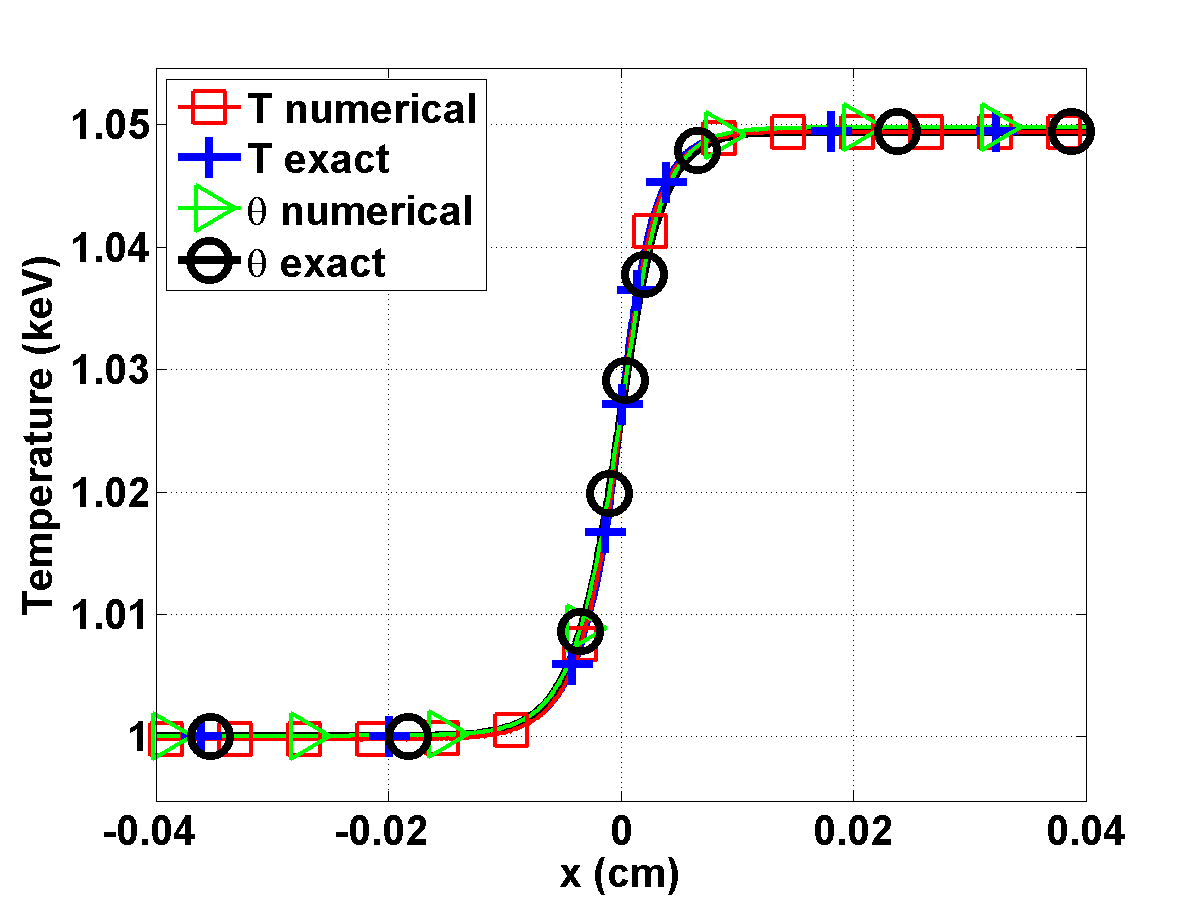
\includegraphics[width=0.3\textwidth]{figures/Mach_1p05_nel_500_temperature.png}
}
\subfigure[Material density]{
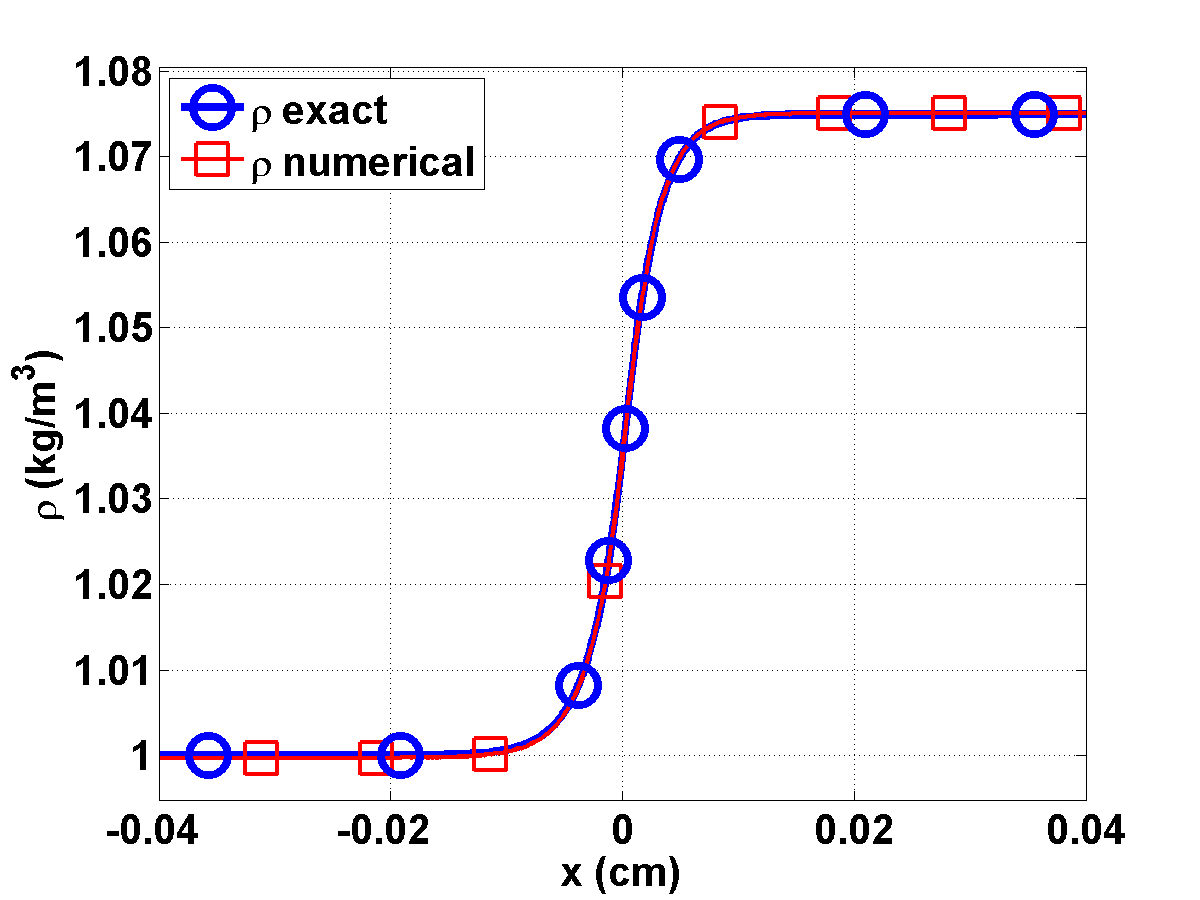
\includegraphics[width=0.3\textwidth]{figures/Mach_1p05_nel_500_density.png}
}
\subfigure[Viscosity coefficient]{
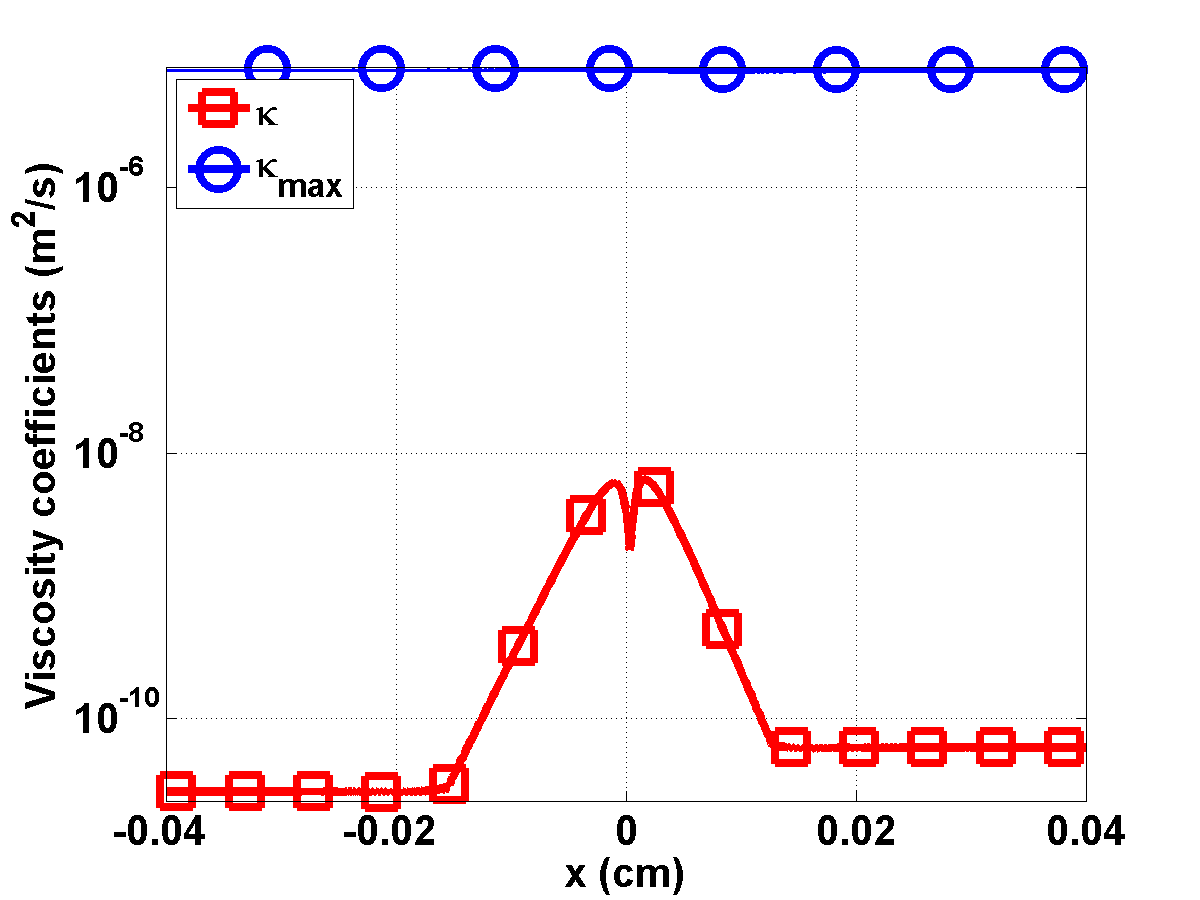
\includegraphics[width=0.3\textwidth]{figures/Mach_1p05_nel_500_viscosity.png}
}
\end{figure}

\end{frame}
%%%%%%%%%%%%%%%%%%%%%%%%%%%%%%%%%%%%%%%%%%%%%%%%%%%%%%%%%%%%%%%%%%%%


%%%%%%%%%%%%%%%%%%%%%%%%%%%%%%%%%%%%%%%%%%%%%%%%%%%%%%%%%%%%%%%%%%%%
\begin{frame}{Steady-state solution for Mach 2}

\begin{figure}[H]
\centering
\subfigure[Temperatures]{
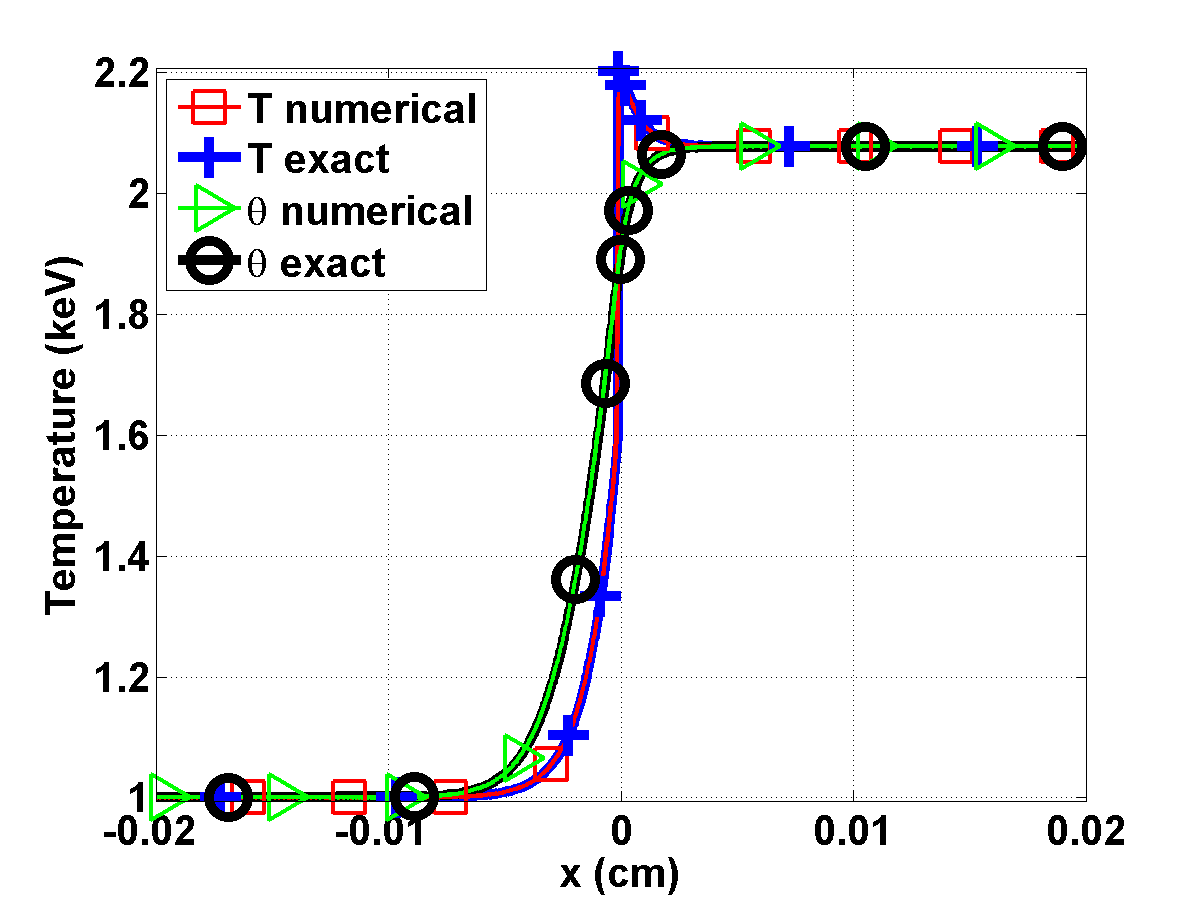
\includegraphics[width=0.3\textwidth]{figures/Mach_2_nel_2000_temperature.png}
}
\subfigure[Material density]{
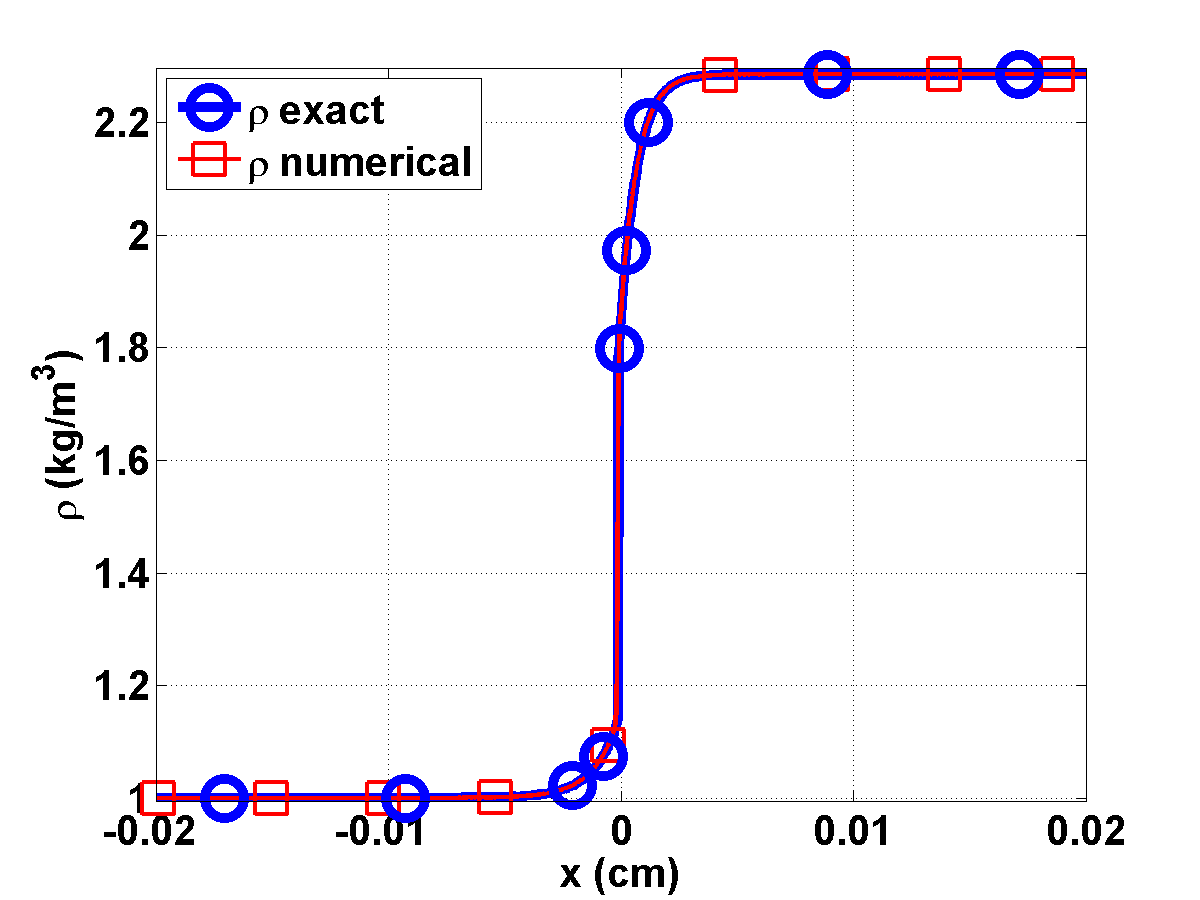
\includegraphics[width=0.3\textwidth]{figures/Mach_2_nel_2000_density.png}
}
\subfigure[Viscosity coefficient]{
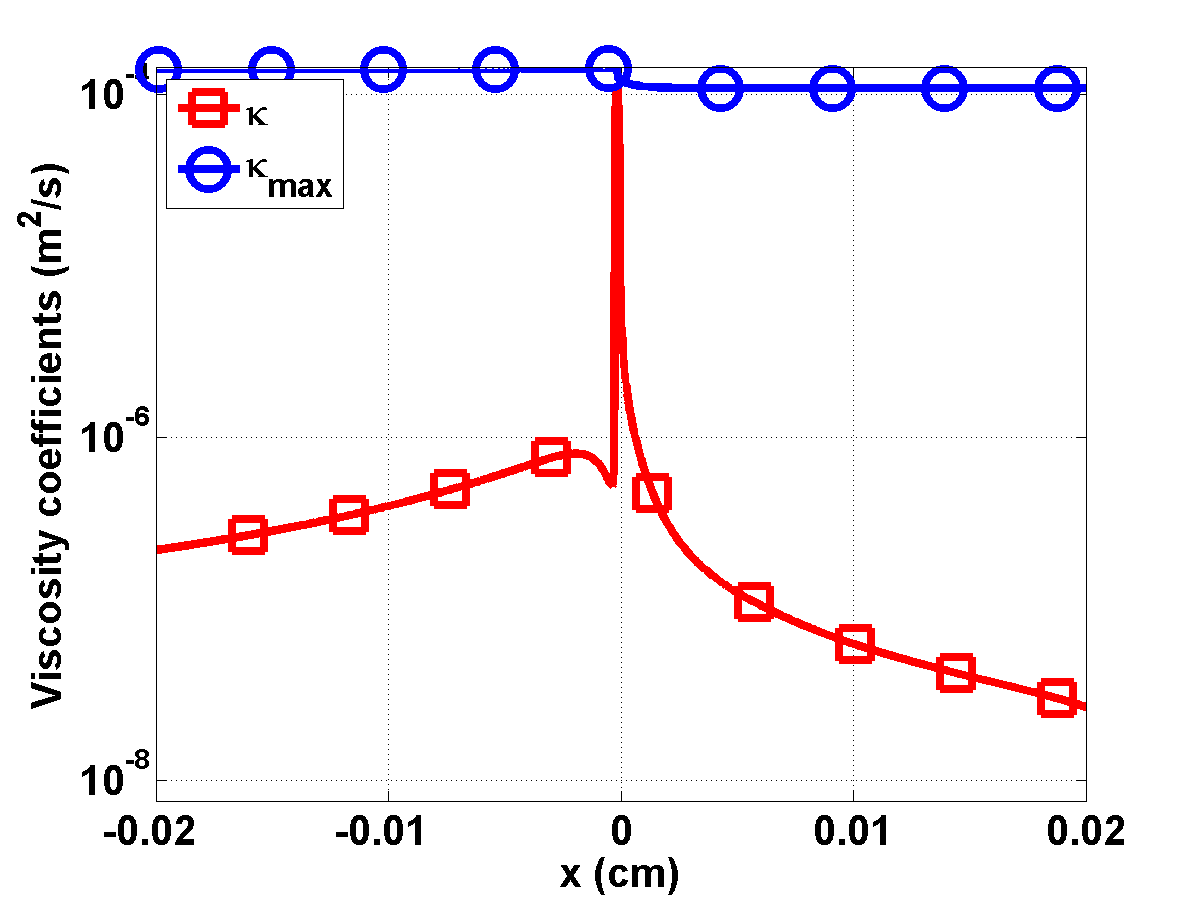
\includegraphics[width=0.3\textwidth]{figures/Mach_2_nel_2000_viscosity.png}
}
\end{figure}

\end{frame}
%%%%%%%%%%%%%%%%%%%%%%%%%%%%%%%%%%%%%%%%%%%%%%%%%%%%%%%%%%%%%%%%%%%%

%%%%%%%%%%%%%%%%%%%%%%%%%%%%%%%%%%%%%%%%%%%%%%%%%%%%%%%%%%%%%%%%%%%%
\begin{frame}{Steady-state solution for Mach 5}

\begin{figure}[H]
\centering
\subfigure[Temperatures]{
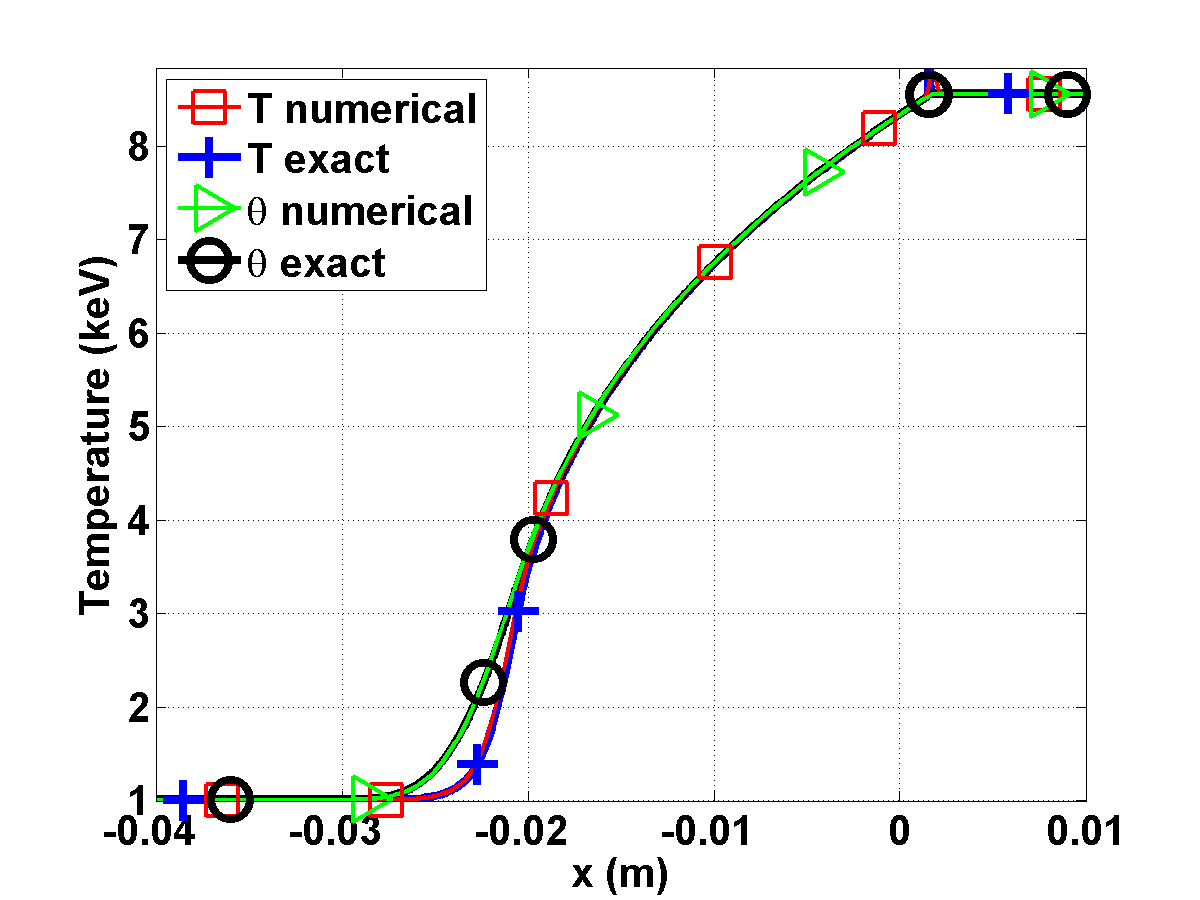
\includegraphics[width=0.3\textwidth]{figures/Mach_5_nel_1000_temperature.png}
}
\subfigure[Material density]{
includegraphics[width=0.3\textwidth]{figures/Mach_5_nel_2000_density.png}
}
\subfigure[Viscosity coefficient]{
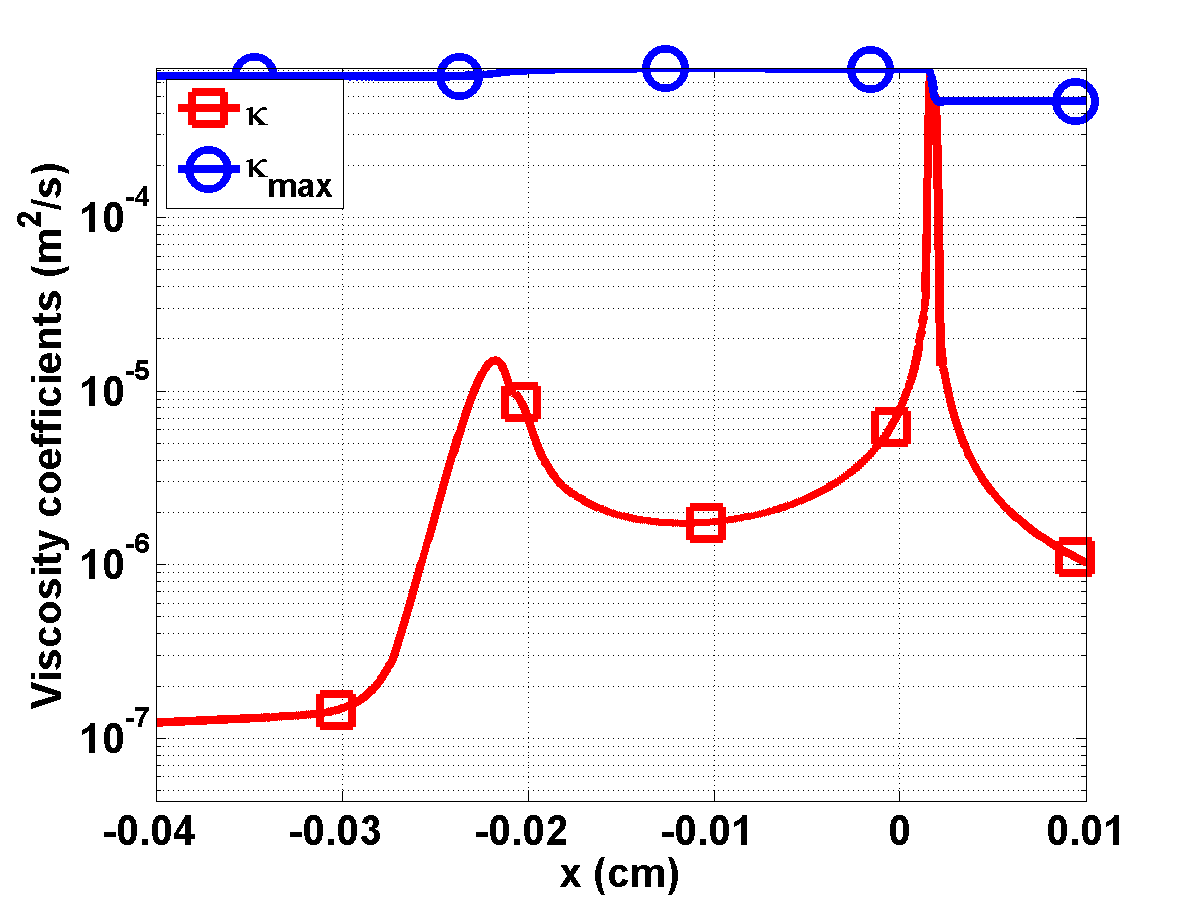
\includegraphics[width=0.3\textwidth]{figures/Mach_5_nel_2000_viscosity.png}
}
\subfigure[Zoom at the Z spike]{
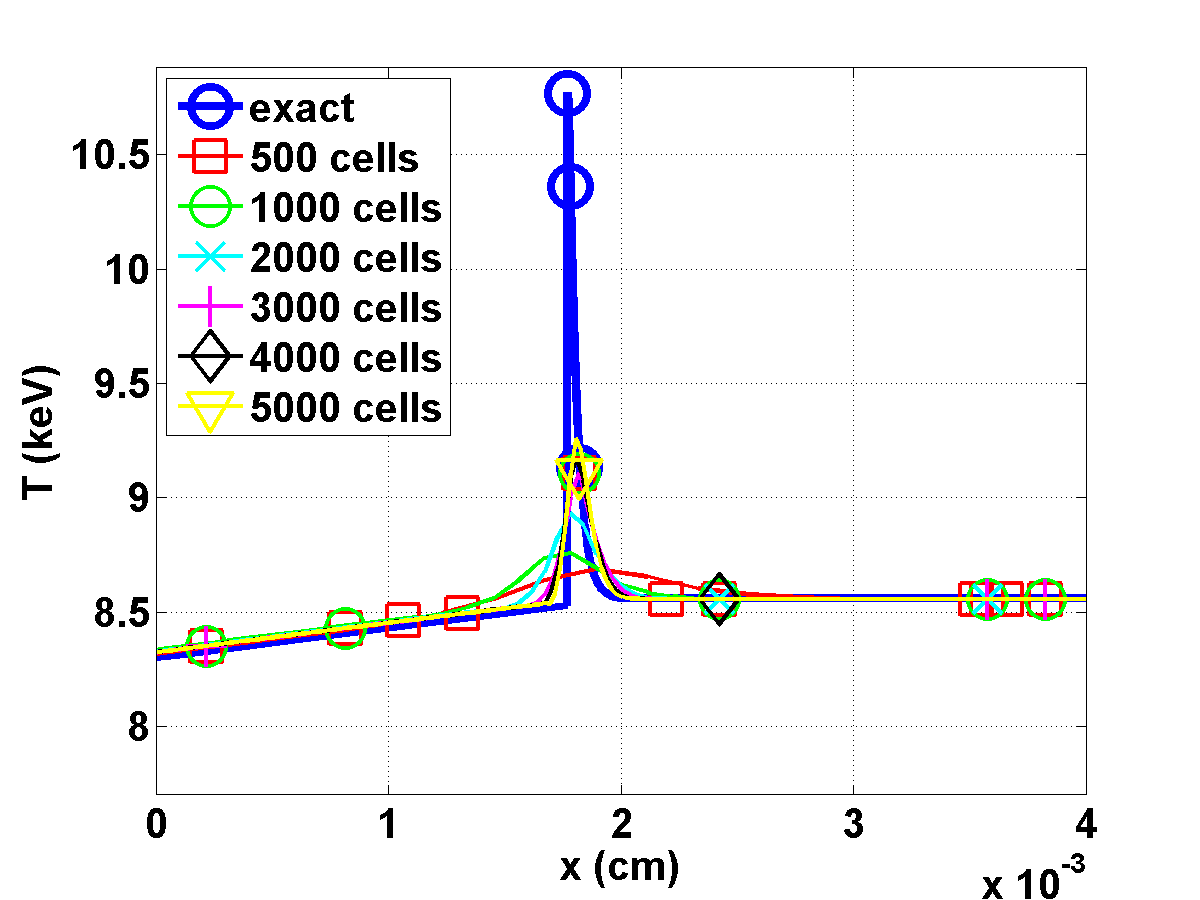
\includegraphics[width=0.3\textwidth]{figures/Mach_5_comparison.png}
}
\end{figure}


\end{frame}
%%%%%%%%%%%%%%%%%%%%%%%%%%%%%%%%%%%%%%%%%%%%%%%%%%%%%%%%%%%%%%%%%%%%

%%%%%%%%%%%%%%%%%%%%%%%%%%%%%%%%%%%%%%%%%%%%%%%%%%%%%%%%%%%%%%%%%%%%
\begin{frame}{Steady-state solution for Mach 50}

\begin{figure}[H]
\centering
\subfigure[Temperatures]{
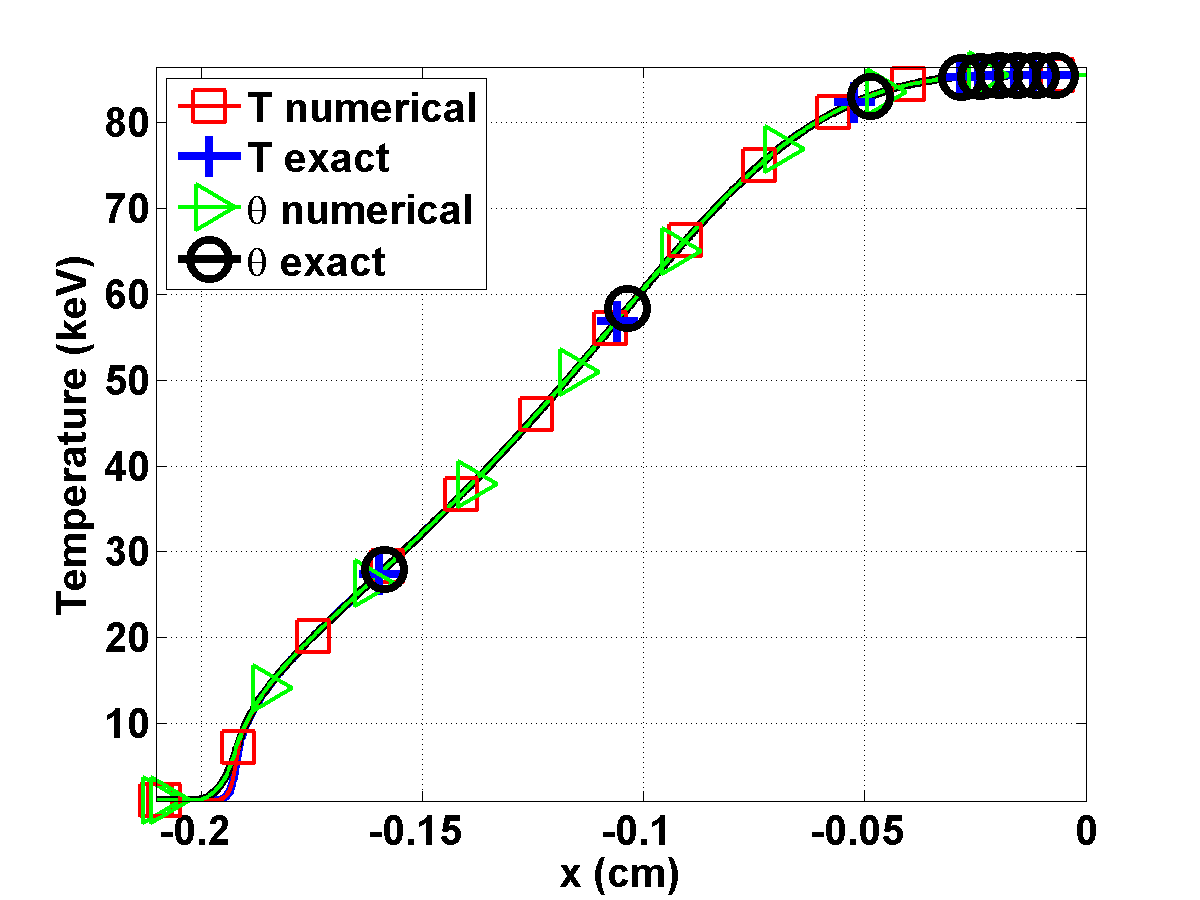
\includegraphics[width=0.3\textwidth]{figures/Mach_50_nel_1000_temperature.png}
}
\subfigure[Material density]{
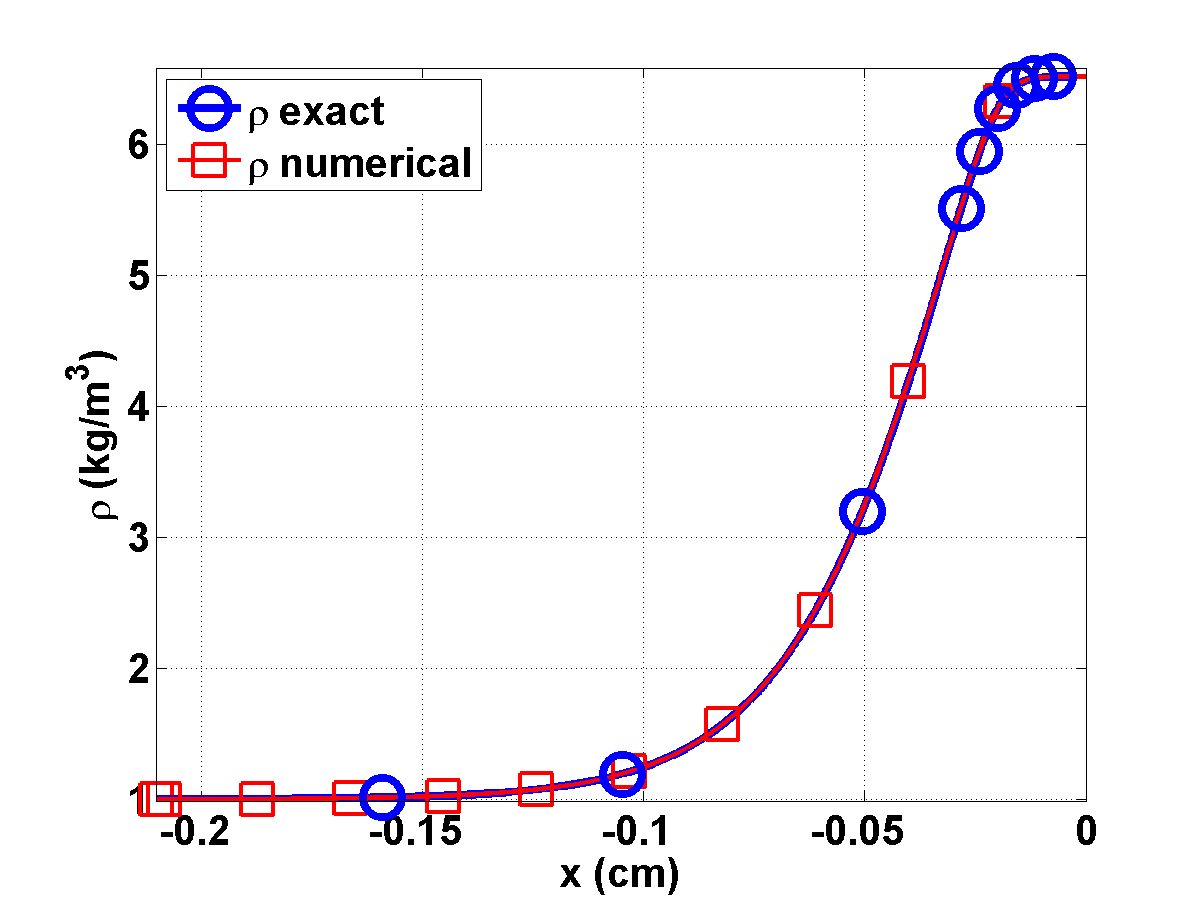
\includegraphics[width=0.3\textwidth]{figures/Mach_50_nel_1000_density.png}
}
\subfigure[Viscosity coefficient]{
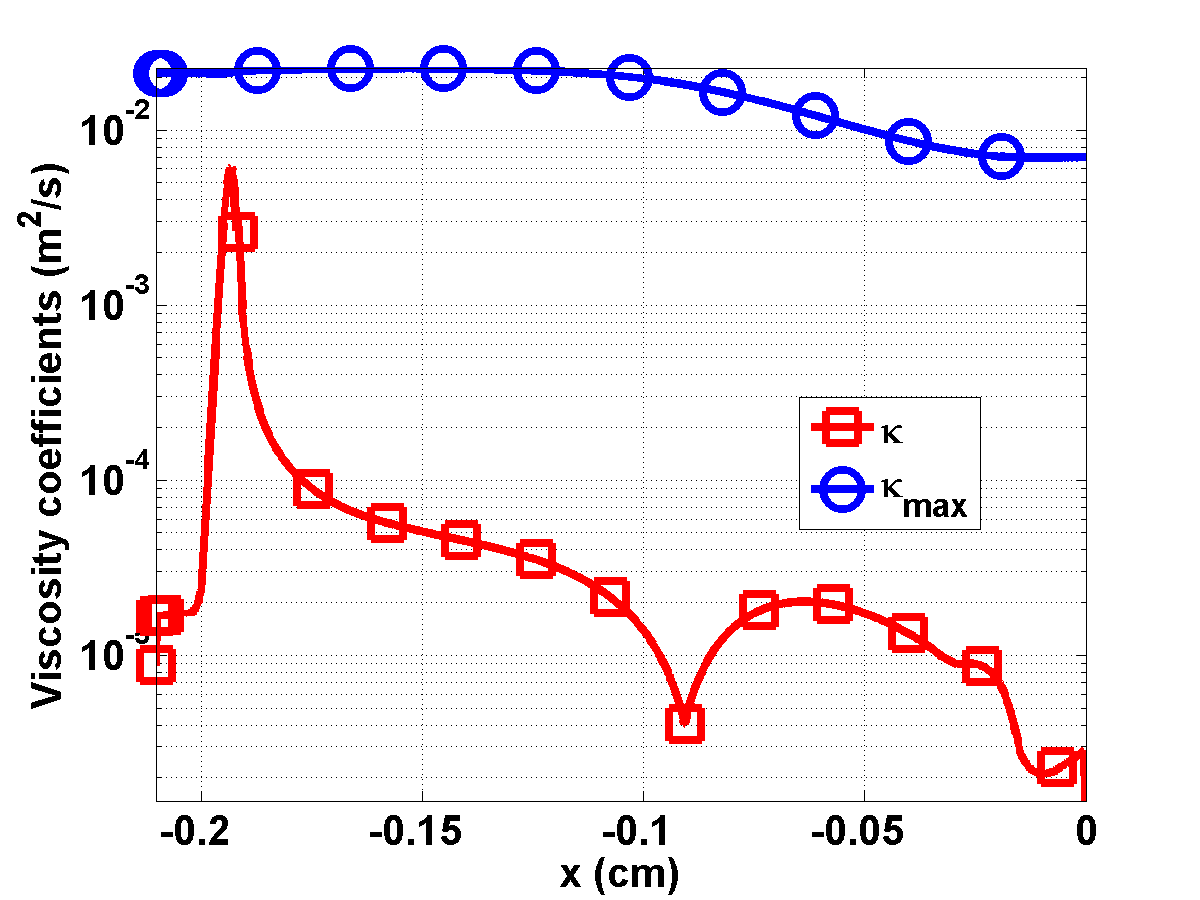
\includegraphics[width=0.3\textwidth]{figures/Mach_50_nel_1000_viscosity.png}
}
\end{figure}

\end{frame}
%%%%%%%%%%%%%%%%%%%%%%%%%%%%%%%%%%%%%%%%%%%%%%%%%%%%%%%%%%%%%%%%%%%%



%%%%%%%%%%%%%%%%%%%%%%%%%%%%%%%%%%%%%%%%%%%%%%%%%%%%%%%%%%%%%%%%%%%%
\begin{frame}{}
\label{lastslide}
\centering
Thank you 

\begin{figure}
	\centering
	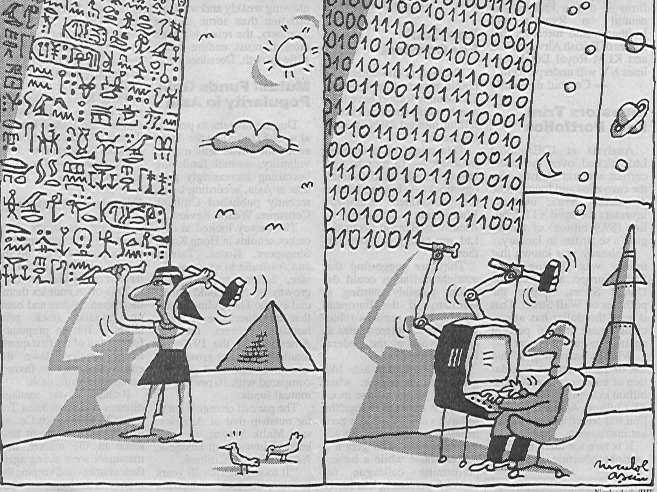
\includegraphics[scale=0.33]{./crunching.png}
\end{figure}

\end{frame}
%%%%%%%%%%%%%%%%%%%%%%%%%%%%%%%%%%%%%%%%%%%%%%%%%%%%%%%%%%%%%%%%%%%%

%%%%%%%%%%%%%%%%%%%%%%%%%%%%%%%%%%%%%%%%%%%%%%%%%%%%%%%%%%%%%%%%%%%%
%%%%%%%%%%%%%%%%%%%%%%%%%%%%%%%%%%%%%%%%%%%%%%%%%%%%%%%%%%%%%%%%%%%%
\section{A Brief Review of the Entropy Viscosity Method for Conservation Laws}
%%%%%%%%%%%%%%%%%%%%%%%%%%%%%%%%%%%%%%%%%%%%%%%%%%%%%%%%%%%%%%%%%%%%
%%%%%%%%%%%%%%%%%%%%%%%%%%%%%%%%%%%%%%%%%%%%%%%%%%%%%%%%%%%%%%%%%%%%

%%%%%%%%%%%%%%%%%%%%%%%%%%%%%%%%%%%%%%%%%%%%%%%%%%%%%%%%%%%%%%%%%%%%
\subsection{Basic Idea}
%%%%%%%%%%%%%%%%%%%%%%%%%%%%%%%%%%%%%%%%%%%%%%%%%%%%%%%%%%%%%%%%%%%%


%%%%%%%%%%%%%%%%%%%%%%%%%%%%%%%%%%%%%%%%%%%%%%%%%%%%%%%%%%%%%%%%%%%%
\begin{frame} 
\frametitle{Quick overview of the entropy-based artificial viscosity formalism}

General scalar conservation law: $\boxed{\partial_t u + \div \vec{f}(u) = 0}$.

\begin{enumerate}
\item 
Add viscous fluxes $\boxed{\partial_t u + \div \vec{f}(u) = \div \mu \grad u}$
\item 
Let the amount of {\bf artificial viscosity} $\mu$ be $\propto$ the {\bf local entropy production}
\begin{itemize}
\item 
Determine an entropy pair ($s(u),\, \vec{\Psi}(u)$) for the PDE under consideration
\item 
Compute the entropy residual $\boxed{R_e:=\partial_t s(u_h) + \div \Psi(u_h)}$, in each cell $K$, at each quadrature point $x_q$
\item 
Compute the speed and kinematic viscosity associated with this residual
\be
v^K_e(x_q)  := h_K \frac{|R_e(x_q)|_K}{|s-\overline{s}|_\infty}
\quad \text{and} \quad 
\mu^K_e(x_q):= h_K v^K_e(x_q) 
\ee
%The denominator is used to normalize the residual
%. It is the deviation of $E(u)$ from the domain average $\overline{E}$.
\end{itemize}
\item 
Limit the viscosity upper bound to the LLF viscosity
\be
\mu^K(x_q) := \min \Big( \frac{h_K}{2} \max_{x\in K}|\vec{f}'(u(x))|, \, \mu^K_e(x_q) \Big)
\ee
\item 
Plug in the standard Galerkin weak form as a \tcm{viscous regularization} %(\tcm{it is really a straightforward technique})
\be
\int_V \big( \partial_t u_h + \div \vec{f}(u_h) \big) b \, dx + \tcm{\sum_K \int_K \mu^K \grad u_h \grad b \, dx} = 0 \quad \forall b
\ee
\end{enumerate}


\end{frame}
%%%%%%%%%%%%%%%%%%%%%%%%%%%%%%%%%%%%%%%%%%%%%%%%%%%%%%%%%%%%%%%%%%%%


%%%%%%%%%%%%%%%%%%%%%%%%%%%%%%%%%%%%%%%%%%%%%%%%%%%%%%%%%%%%%%%%%%%%
\begin{frame}{Why an upper bound for viscosity?}

\begin{block}{}
Large entropy residual in shocks $\longrightarrow$ large entropy viscosity $\mu_e$ \\
\begin{center}
There is such a thing as too much of a good thing ...\\
{\it Il ne faut point \^{e}tre plus royaliste que le Roy}
\end{center}
\end{block}


\begin{block}{Upper bound for $\mu$}
First-order upwind scheme is monotone but over dissipative. We should not exceed the amount of stabilization that such a scheme provides.\\
\medskip
upwinding = \textcolor{blue}{centered approximation (Galerkin)} $-$ \textcolor{magenta}{numerical diffusion}\\
\underline{Example: linear advection} $\partial_t u + \beta \partial_x u =0$
\be
\beta \frac{u_i - u_{i-1}}{h} = \textcolor{blue}{\beta\frac{ u_{i+1}- u_{i-1}}{2h}} - \textcolor{red}{\frac{\beta h}{2}}
\textcolor{magenta}{\frac{ u_{i+1}-2u_i +u_{i-1}}{h^2}}
\ee
So, the dissipative term is $\frac{\beta h}{2}\partial_{xx} u$
and the first-order viscosity is $\frac{\beta h}{2}$
\end{block}

\begin{block}{First-order viscosity}
\hspace{0.5cm} $\bullet$ scalar conservation law: $\frac{h}{2}|f'(u)|$
\hspace{0.5cm} $\bullet$ system: $\frac{h}{2} \max \left( \text{eig}( \partial_u f) \right) $
\end{block}


\end{frame}
%%%%%%%%%%%%%%%%%%%%%%%%%%%%%%%%%%%%%%%%%%%%%%%%%%%%%%%%%%%%%%%%%%%%


%%%%%%%%%%%%%%%%%%%%%%%%%%%%%%%%%%%%%%%%%%%%%%%%%%%%%%%%%%%%%%%%%%%%
%\begin{frame} 
%\frametitle{Example: Burgers equation}
%\begin{figure}
%	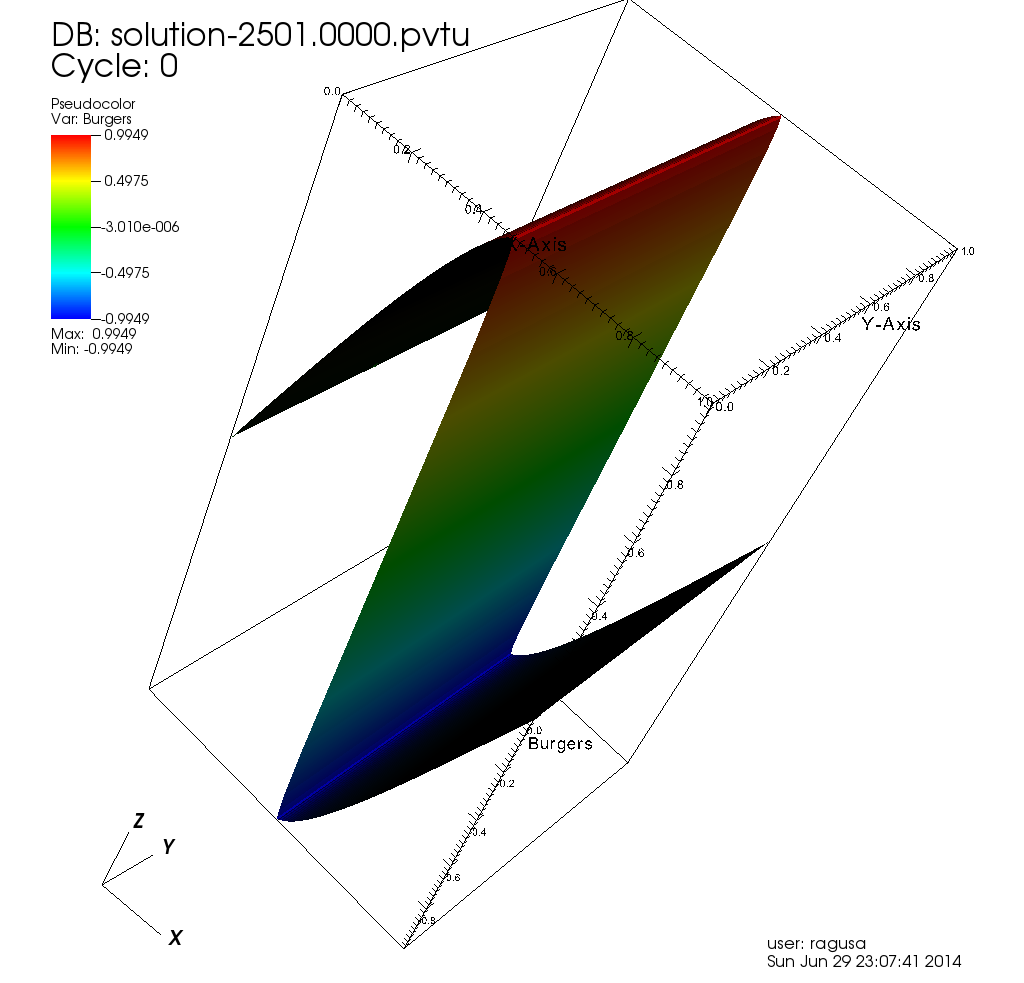
\includegraphics[height=7cm, keepaspectratio=true]{figs/burgers0000.png}
%\end{figure}
%\end{frame}
%
%\begin{frame} 
%\begin{figure}
%	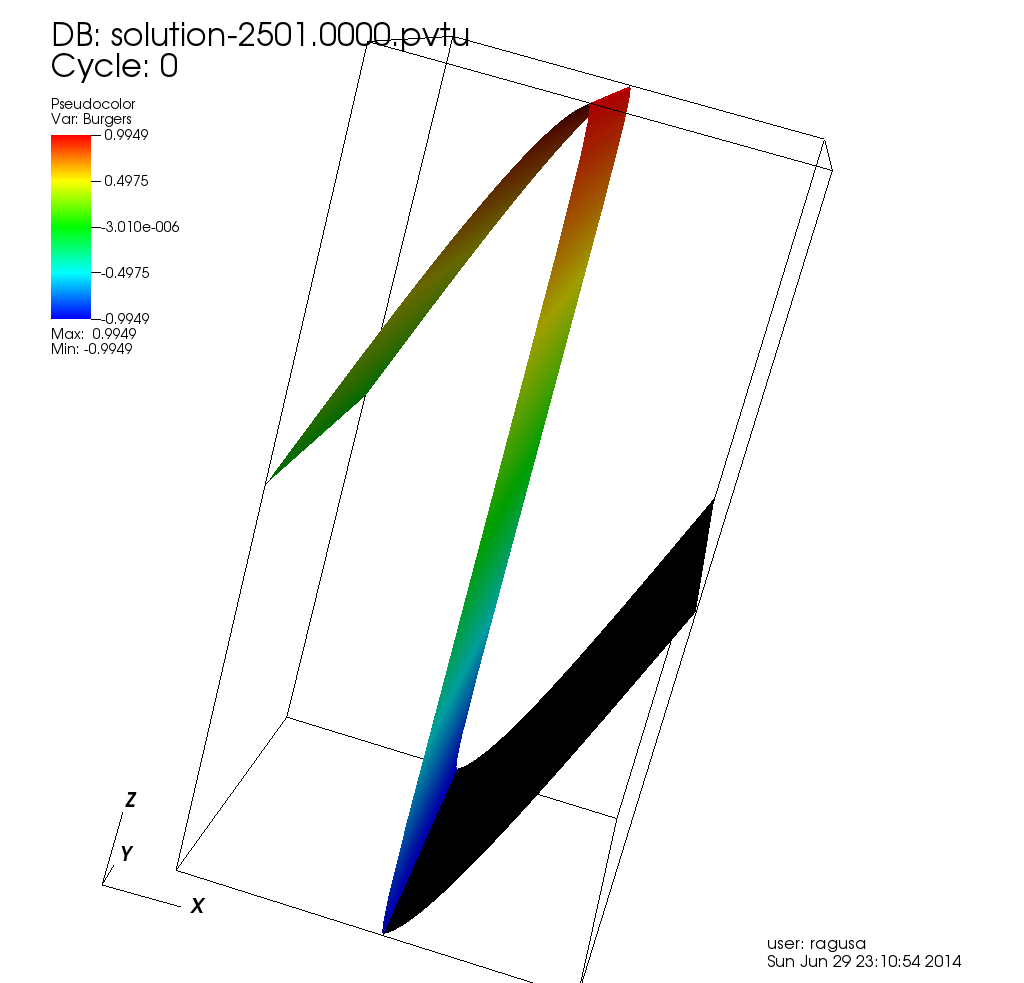
\includegraphics[height=7cm, keepaspectratio=true]{figs/burgers20000.png}
%\end{figure}
%\end{frame}

\begin{frame}
\frametitle{Example: Burgers equation}
\begin{figure}
        \centering
        \begin{subfigure}[b]{0.37\textwidth}
                \centering
                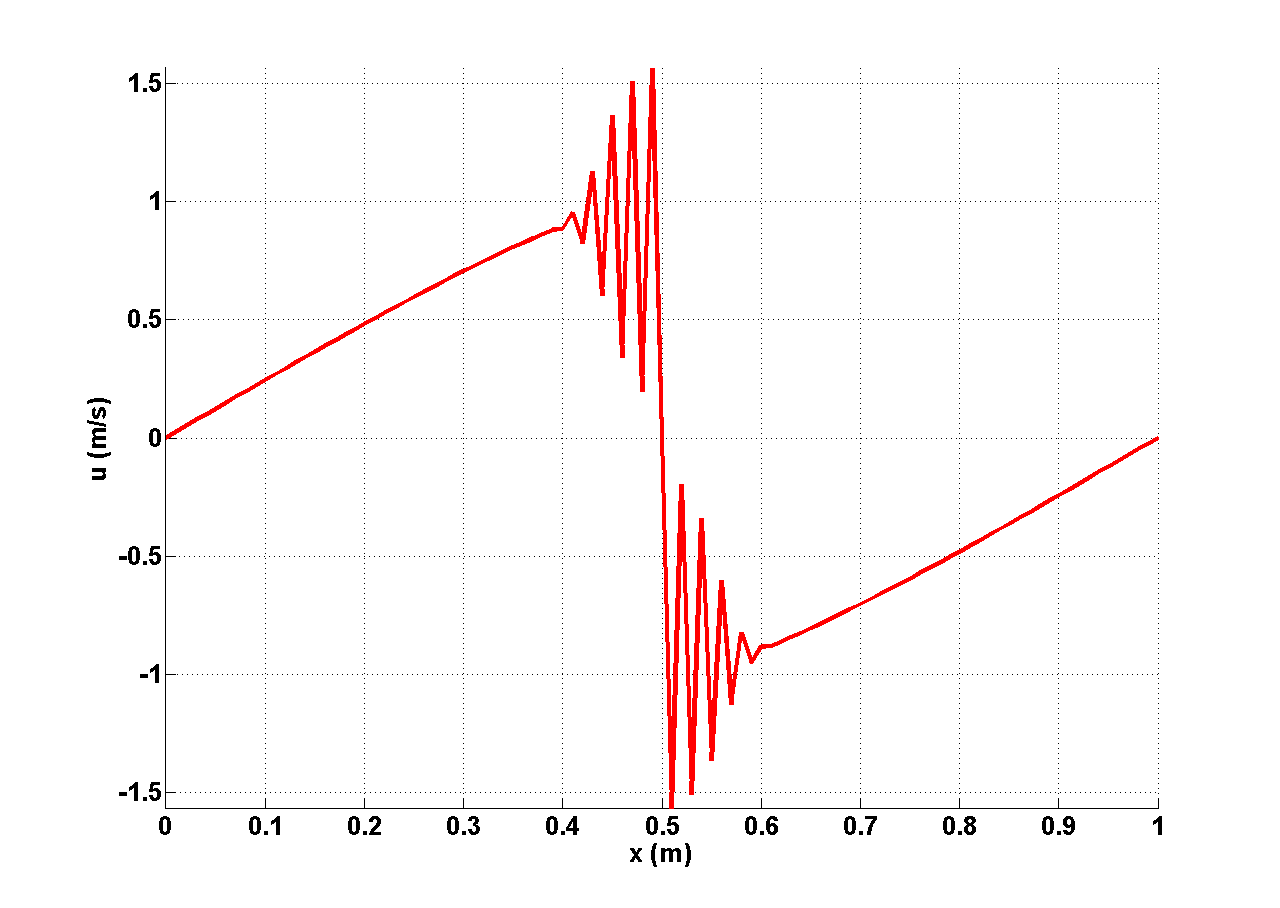
\includegraphics[width=\textwidth]{figs/1D_sol_free.png}
                \caption{Without stabilization.}
        \end{subfigure}%
        \begin{subfigure}[b]{0.37\textwidth}
                \centering
                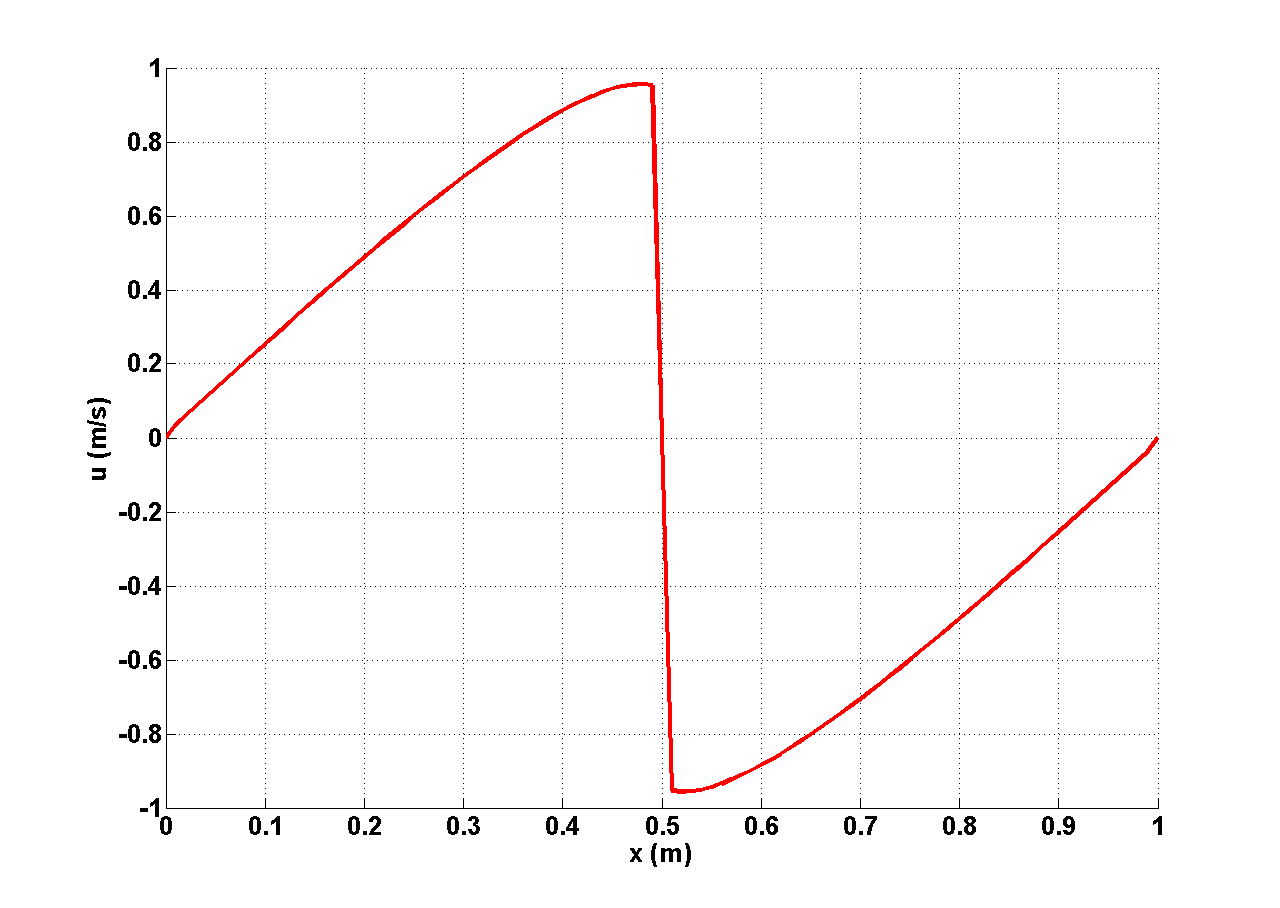
\includegraphics[width=\textwidth]{figs/1D_sol_fo.png}
                \caption{With first-order viscosity.}
        \end{subfigure}
        
        \begin{subfigure}[b]{0.37\textwidth}
                \centering
                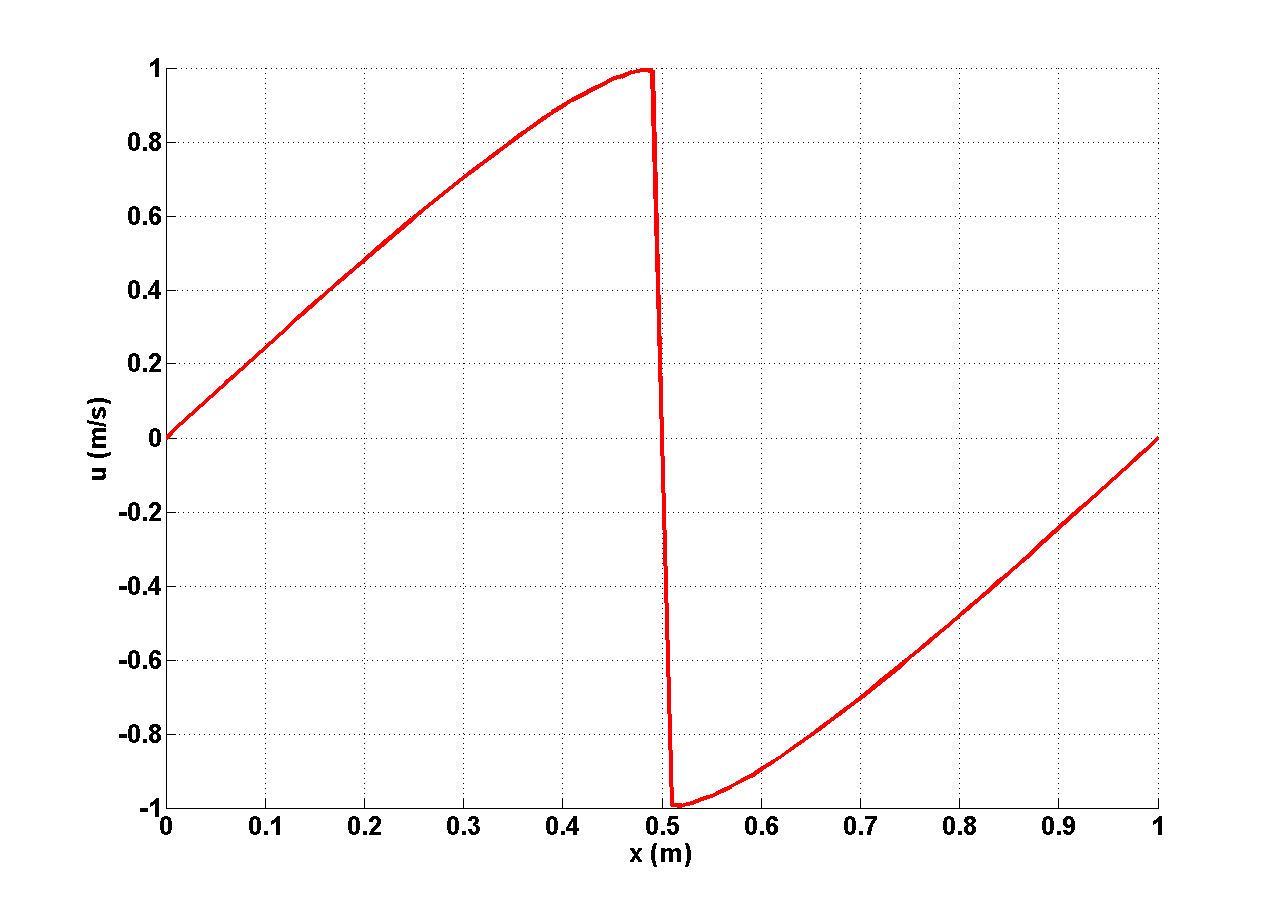
\includegraphics[width=\textwidth]{figs/1D_sol_ev.png}
                \caption{With the EVM.}
        \end{subfigure}
        \begin{subfigure}[b]{0.37\textwidth}
                \centering
                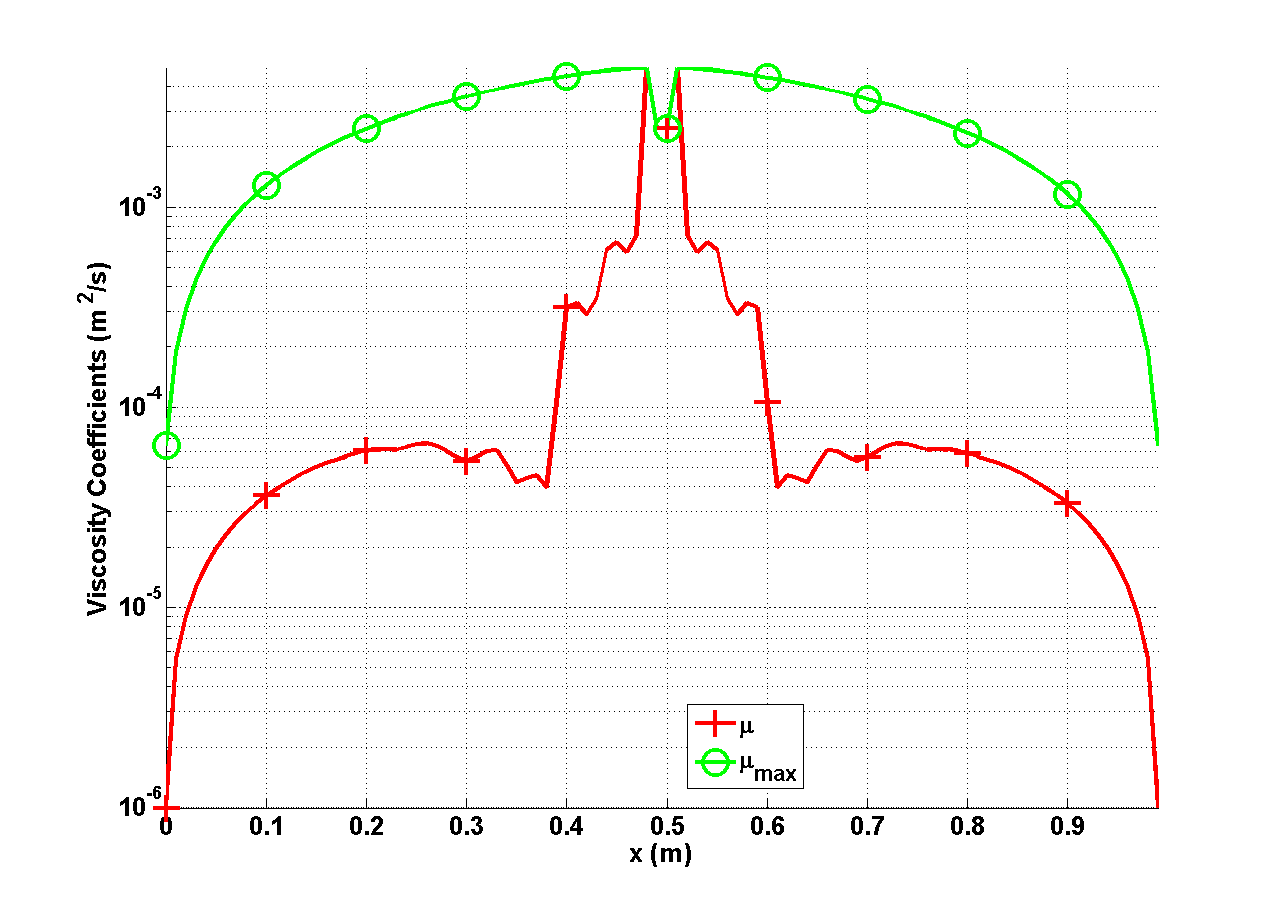
\includegraphics[width=\textwidth]{figs/1D_visc.png}
                \caption{Viscosity coefficient profiles.}
        \end{subfigure}
\end{figure}
\end{frame}
%%%%%%%%%%%%%%%%%%%%%%%%%%%%%%%%%%%%%%%%%%%%%%%%%%%%%%%%%%%%%%%%%%%%


%%%%%%%%%%%%%%%%%%%%%%%%%%%%%%%%%%%%%%%%%%%%%%%%%%%%%%%%%%%%%%%%%%%%
\subsection{Application to the Entropy Viscosity Method to the Euler Equations}
%%%%%%%%%%%%%%%%%%%%%%%%%%%%%%%%%%%%%%%%%%%%%%%%%%%%%%%%%%%%%%%%%%%%

%%%%%%%%%%%%%%%%%%%%%%%%%%%%%%%%%%%%%%%%%%%%%%%%%%%%%%%%%%%%%%%%%%%%
%************************************************
\subsection{Entropy-viscosity method: original supersonic formulation}
%%************************************************

%%%%%%%%%%%%%%%%%%%%%%%%%%%%%%%%%%%%%%%%%%%%%%%%%%%%%%%%%%%%%%%%%%%%
\begin{frame}
\begin{block}{\tcr{Regularized} Euler equations}
\begin{subequations}
\label{eq:euler_visc}
%
\begin{equation}
\partial_t \rho + \div \left( \rho \vec{u} \right) = \textcolor{red}{\div \vec{f}} \nonumber
\end{equation}
%
\begin{equation}
\partial_t \left( \rho \vec{u} \right) + \div \left( \rho \vec{u} \otimes \vec{u} + P \mathbb{I} \right) =  \textcolor{red}{\div \mathbb{g} }\nonumber
\end{equation}
%
\begin{equation}
\partial_t \left( \rho E  \right) + \div \left[ \vec{u} \left( \rho E + P \right) \right] = \textcolor{red}{\div \vec{h} }\nonumber
\end{equation}
\end{subequations}

\smallskip

How to determine the \tcr{artificial viscous fluxes}?

\smallskip

By proving that the regularized equations satisfy a minimum principle on the specific entropy

\end{block}

\begin{block}{Minimum entropy principle}
\be
\inf_{x\in \mathbb{R}^d} s(x,t) \ge \inf_{x\in \mathbb{R}^d} s_0(x) \qquad \forall t \ge 0
\ee
\end{block}

\end{frame}
%%%%%%%%%%%%%%%%%%%%%%%%%%%%%%%%%%%%%%%%%%%%%%%%%%%%%%%%%%%%%%%%%%%%


%%%%%%%%%%%%%%%%%%%%%%%%%%%%%%%%%%%%%%%%%%%%%%%%%%%%%%%%%%%%%%%%%%%%
\begin{frame}{Idea of the derivation}

\begin{block}{Entropy relationship: $\partial_t s + \vec{u} \cdot \grad s = \ldots $}
Entropy is a function of internal energy $e$ and density $\rho$. Using chain rule, we have
\[
\partial_\alpha s = s_\rho \partial_\alpha \rho + s_e \partial_\alpha e \quad \text{ with } \alpha={t,x}
\]
Re-write Euler equations in non-conservative form as a function of $\rho$, $u$, and $e$
\end{block}

\begin{block}{Entropy equation}
Use chain rule and the mass and internal energy equations to get:
\begin{align}
\rho \left( \partial_t s + \mbold{u} \cdot \grad s \right) = \div \left( \rho \kappa \grad s \right) -  \kappa \rho \mathbf{Q} +  s_e \mu \grad^s \mbold{u} : \grad \mbold{u} \nonumber
\end{align}
\end{block}
%
\begin{block}{Quadratic form}
\begin{equation}
\mathbf{Q} = X^t \mathbb{\Sigma} X 
\quad \text{ with } 
X = 
\begin{bmatrix}
\grad \rho \\
\grad e 
\end{bmatrix}
\text{ and } 
\mathbb{\Sigma} = 
\begin{bmatrix}
       \partial_{\rho} (\rho^2 \partial_{\rho} s) & \partial_{\rho,e} s  \\[0.3em]
       \partial_{\rho,e} s & \partial_{e,e} s           \\[0.3em]
\end{bmatrix} \nonumber 
\end{equation}
The form $Q$ is negative definite if and only if $-s$ is convex with respect to $e$ and $\rho^{-1}$.
\end{block}
\tcr{QED} \ \ (recall: $s_e = 1/T > 0 $)

\end{frame}
%%%%%%%%%%%%%%%%%%%%%%%%%%%%%%%%%%%%%%%%%%%%%%%%%%%%%%%%%%%%%%%%%%%%


%%%%%%%%%%%%%%%%%%%%%%%%%%%%%%%%%%%%%%%%%%%%%%%%%%%%%%%%%%%%%%%%%%%%
\begin{frame}
\begin{block}{Euler equations with viscous regularization (final form)}
\begin{subequations}
\label{eq:euler_visc}
%
%\text{Continuity equation:}
\begin{equation}
\partial_t \rho + \div \left( \rho \vec{u} \right) = \textcolor{red}{\div \left( \kappa  \grad \rho \right)} \nonumber
\end{equation}
%
%\text{Momentum equation:}
\begin{equation}
\partial_t \left( \rho \vec{u} \right) + \div \left( \rho \vec{u} \otimes \vec{u} + P \mathbb{I} \right) =  \textcolor{red}{\div \left( \mu \rho  \grad^s \vec{u}  + \kappa \vec{u} \otimes \grad \rho \right) }\nonumber
\end{equation}
%
%\text{Energy equation:}
\begin{equation}
\partial_t \left( \rho E  \right) + \div \left[ \vec{u} \left( \rho E + P \right) \right] = \textcolor{red}{\div \left( \kappa \grad \left( \rho e \right) + \frac{1}{2}|| \vec{u} ||^2 \kappa \grad \rho +  \rho \mu \vec{u} \grad \vec{u}  \right) }\nonumber
\end{equation}
\end{subequations}

\smallskip

where $\kappa$ and $\mu$ are positive viscosity coefficients.
\end{block}

Note that if $\mu = \kappa$ (and one selects $\grad \vec{u} $ instead of $\grad^s \vec{u} $), we recover a parabolic regularization (on $\rho$, $\rho \vec{u}$, and $\rho E$).

%\begin{block}{}
%\hspace{0.5cm} $\bullet$ Multi-wave problem: $\lambda_1 = \vec{u} \cdot \vec{n} - c $, $\lambda_2 = \vec{u} \cdot \vec{n} + c $ and $\lambda_{3, \dots, 3+D} = \vec{u} \cdot \vec{n}$. \\
%\hspace{0.5cm} $\bullet$ $\kappa$ and $\mu$ are two positive viscosity coefficients.
%\end{block}
\end{frame}
%%%%%%%%%%%%%%%%%%%%%%%%%%%%%%%%%%%%%%%%%%%%%%%%%%%%%%%%%%%%%%%%%%%%



%%%%%%%%%%%%%%%%%%%%%%%%%%%%%%%%%%%%%%%%%%%%%%%%%%%%%%%%%%%%%%%%%%%%
\begin{frame} 
\frametitle{Mach-3 forward facing step: density contour}

\begin{center}
\movie[width=6cm,height=4cm,showcontrols=true,externalviewer]{
\includegraphics[width=6cm,height=4cm]{engr.pdf}}{movs/forward_facing_step_density_movie.mpeg}\\
\end{center}

%\begin{center}
  %\begin{columns}
    %\column{.5\textwidth}
       %\includemedia[addresource=compression_corner.mp4, activate=pageopen, deactivate=pageclose, width=6.5cm, height=5cm, flashvars={source=mov/compression_corner.mp4 & autoPlay=true & loop=true }]{}{VPlayer.swf}
    %\column{.5\textwidth}
      %\includemedia[addresource=compression_corner_viscosity.mp4, activate=pageopen, deactivate=pageclose, width=6.5cm, height=5cm, flashvars={source=mov/compression_corner_viscosity.mp4 & autoPlay=true & loop=true }]{}{VPlayer.swf}
  %\end{columns}
%\end{center}


\end{frame}
\begin{frame} 
\frametitle{Mach-3 forward facing step: viscosity contour}

\begin{center}
\movie[width=6cm,height=4cm,showcontrols=true,externalviewer]{
\includegraphics[width=6cm,height=4cm]{engr.pdf}}{movs/forward_facing_step_viscosity.mpeg}\\
\end{center}

\end{frame}
%%%%%%%%%%%%%%%%%%%%%%%%%%%%%%%%%%%%%%%%%%%%%%%%%%%%%%%%%%%%%%%%%%%%


%%%%%%%%%%%%%%%%%%%%%%%%%%%%%%%%%%%%%%%%%%%%%%%%%%%%%%%%%%%%%%%%%%%%
%%%%%%%%%%%%%%%%%%%%%%%%%%%%%%%%%%%%%%%%%%%%%%%%%%%%%%%%%%%%%%%%%%%%
\section{Extension of the Entropy Viscosity Method to Low-Mach Flows}
%%%%%%%%%%%%%%%%%%%%%%%%%%%%%%%%%%%%%%%%%%%%%%%%%%%%%%%%%%%%%%%%%%%%
%%%%%%%%%%%%%%%%%%%%%%%%%%%%%%%%%%%%%%%%%%%%%%%%%%%%%%%%%%%%%%%%%%%%

%%%%%%%%%%%%%%%%%%%%%%%%%%%%%%%%%%%%%%%%%%%%%%%%%%%%%%%%%%%%%%%%%%%%
\subsection{New Formulation of the Entropy Residual}
%%%%%%%%%%%%%%%%%%%%%%%%%%%%%%%%%%%%%%%%%%%%%%%%%%%%%%%%%%%%%%%%%%%%


%%%%%%%%%%%%%%%%%%%%%%%%%%%%%%%%%%%%%%%%%%%%%%%%%%%%%%%%%%%%%%%%%%%%
\begin{frame} 
\frametitle{\textcolor{red}{Low-Mach issues} with current viscosity definitions}

Recall that 

\begin{equation}
\mu^K_e(\vec{r}_q,t) =  h_K^2 \frac{|\resi^K(\vec{r}_q,t) |}{\textcolor{magenta}{|| s - \bar{s} ||_\infty}} 
%\qquad
%\kappa^K_e(\vec{r}_q,t) = \Pr \, \mu^K_e(\vec{r}_q,t)
\end{equation}


\begin{block}{Issues with current formulation in the low-Mach limit}
\begin{itemize}
\item In the low-Mach Regime, the flow is known to be \textcolor{red}{isentropic}, resulting in very little entropy production
\item In practice, the entropy residual $\resi$ will be very small in that regime  (i.e., small numerator in the expression for the viscosity coefficients)
\item and so will be the denominator $|| s - \bar{s} ||_\infty$,
\item Thus, the formula for the viscosity coefficients are not determined \textcolor{red}{(ill-scaled) in the low-Mach limit}
\end{itemize}
\end{block}

\end{frame}

%%%%%%%%%%%%%%%%%%%%%%%%%%%%%%%%%%%%%%%%%%%%%%%%%%%%%%%%%%%%%%%%%%%%

%%%%%%%%%%%%%%%%%%%%%%%%%%%%%%%%%%%%%%%%%%%%%%%%%%%%%%%%%%%%%%%%%%%%
\begin{frame} 
\frametitle{Alternate definition of the entropy residual}

We can show that
\begin{equation}
\label{eq:ent_res}
\resi(\vec{r},t) := \partial_t s + \vec{u} \cdot \grad s = \matder{s} = \frac{s_e}{P_e} \underbrace{\left( \matder{P} - c^2 \matder{\rho} \right)}_{\resinew(\vec{r},t)} 
\end{equation} 

Idea for the demonstration: 
$s$ is a function of $e$ and $\rho$, thus $\matder{s} = s_e\matder{e} + s_\rho \matder{\rho}$\\
Re-express the internal energy $e$ as a function of $P$ and $\rho$ through the EoS.

\begin{block}{Consequences}
\begin{itemize}
\item Residuals $\resi$ and $\resinew$ are proportional to one another %and will experience similar variations in space and time. 
\item We elect to employ $\resinew$ instead of $\resi$ %for the evaluation of the local entropy residual.
\item {\it An analytical expression of the entropy function $s$ is no longer needed} %: the residual $\resinew$ is evaluated using the local values of $P\,,\rho\,,u\,,c$ %pressure, density, velocity and speed of sound.
\item \textcolor{red}{Suitable normalizations for the residual} $\resinew$ can be devised (e.g., $P$, $\rho c^2$, $\rho c || \vec{u} ||$ or $\rho || \vec{u} ||^2$)%. Examples include the pressure itself or combinations of the density, the speed of sound and the norm of the velocity, i.e., $\rho c^2$, $\rho c || \vec{u} ||$ or $\rho || \vec{u} ||^2$. 
\end{itemize}
\end{block}


%\begin{block}{What is a proper normalization for $\resinew(\vec{r},t)$?}
%Requirements
%\begin{enumerate}
%\item To recover the incompressible results in the low-Mach limit %(i.e., pressure fluctuations $\propto M^2$; divergence-free flow; incompressible continuity equation)
%\item To remain valid and accurate for supersonic flows
%\end{enumerate}
%\textcolor{red}{Asymptotic analysis} to determine the proper scaling in the low-Mach limit.
%
%\end{block}

\end{frame}
%%%%%%%%%%%%%%%%%%%%%%%%%%%%%%%%%%%%%%%%%%%%%%%%%%%%%%%%%%%%%%%%%%%%





%%%%%%%%%%%%%%%%%%%%%%%%%%%%%%%%%%%%%%%%%%%%%%%%%%%%%%%%%%%%%%%%%%%%
\begin{frame} 
\frametitle{What is a proper normalization for $\resinew(\vec{r},t)$?}

\begin{block}{Requirements} % {What is a proper normalization for $\resinew(\vec{r},t)$?}
\begin{enumerate}
\item To recover the incompressible results in the low-Mach limit (i.e., pressure fluctuations $\propto M^2$; divergence-free flow; incompressible continuity equation)
\item To remain valid and accurate for supersonic flows
\end{enumerate}

\end{block}

\smallskip 

We pose
\begin{equation}
\mu^K_e(\vec{r}_q,t)    = h_K^2 \frac{ | \resinew^K(\vec{r}_q,t) | }{\norm_P^\mu}    
%\end{equation} 
\quad
\text{and} 
\quad
%\begin{equation}
\kappa^K_e(\vec{r}_q,t) = h_K^2 \frac{ | \resinew^K(\vec{r}_q,t) | }{\norm_P^\kappa} 
\end{equation}

\bigskip

We now need to determine $\norm_P^\mu$ and $\norm_P^\kappa$. $\longrightarrow$
\textcolor{red}{Asymptotic analysis} to determine the proper scaling in the low-Mach limit.
%\textcolor{red}{Low-Mach Asymptotic analysis}. % to determine the viscosity coefficient scaling in the low-Mach limit.

\end{frame}
%%%%%%%%%%%%%%%%%%%%%%%%%%%%%%%%%%%%%%%%%%%%%%%%%%%%%%%%%%%%%%%%%%%%

%%%%%%%%%%%%%%%%%%%%%%%%%%%%%%%%%%%%%%%%%%%%%%%%%%%%%%%%%%%%%%%%%%%%
\subsection{Low-Mach Asymptotics}
%%%%%%%%%%%%%%%%%%%%%%%%%%%%%%%%%%%%%%%%%%%%%%%%%%%%%%%%%%%%%%%%%%%%

%%%%%%%%%%%%%%%%%%%%%%%%%%%%%%%%%%%%%%%%%%%%%%%%%%%%%%%%%%%%%%%%%%%%
\begin{frame} 
\frametitle{Low-Mach Asymptotics: non-dimensionalization}

\begin{block}{Non-dimensionalized variables}

\begin{multline}
\label{eq:norm_param}
\rho^*   = \frac{\rho}{\rho_\infty}           ,\
u^*      = \frac{u}{u_\infty}                 ,\
P^*      = \frac{P}{\rho_\infty c^2_\infty}   ,\
E^*      = \frac{E}{c^2_\infty }              ,\\
x^* = \frac{x}{L_\infty}                      ,\
t^* = \frac{t}{L_\infty / u_\infty}           ,\ 
\mu^*    = \frac{\mu}{\mu_\infty}             ,\
\kappa^* = \frac{\kappa}{\kappa_\infty}       ,
\end{multline}
%
where  the subscript $\infty$ denote the far-field  quantities and the superscript $*$ stands for the non-dimensionalized variables.

\medskip

%The far-field reference quantities are chosen such that the dimensionless flow quantities are of order 1. 
%
%\medskip

The reference Mach number is given by
%
\begin{equation}
M_\infty = \frac{u_\infty}{c_\infty} ,
\end{equation}

\end{block}

\end{frame}
%%%%%%%%%%%%%%%%%%%%%%%%%%%%%%%%%%%%%%%%%%%%%%%%%%%%%%%%%%%%%%%%%%%%

%%%%%%%%%%%%%%%%%%%%%%%%%%%%%%%%%%%%%%%%%%%%%%%%%%%%%%%%%%%%%%%%%%%%
\begin{frame} 
\frametitle{Scaled Euler equations with viscous regularization}

\begin{subequations} 
\label{eq:Euler_eq2}
%
\begin{equation}
\label{eq:euler_eq2_cont}
\partial_{t^*} \rho^*+ \divv{*}  \left(  \rho^* \vec{u}^*  \right) = \frac{1}{\tcr{\Pe_\infty}} \divv{*}  ( \kappa^* \gradd{*} \rho^* )
\end{equation}
%
\begin{multline}
\label{eq:euler_eq2_mom}
\partial_{t^*} \left( \rho^* \vec{u}^* \right) 
+ \divv{*} \left( \rho^* \vec{u}^*\otimes \vec{u}^* \right) 
+ \frac{1}{\tcr{M_\infty^2}}\gradd{*}  P^*  
= 
\frac{1}{\tcr{\Re_\infty}} \divv{*} \left( \rho^* \mu^* \gradd{s,*} \vec{u}^* \right)  \\
+
\frac{1}{\tcr{\Pe_\infty}} \divv{*} \left(\vec{u}^*\otimes \kappa^* \gradd{*}  \rho^* \right)
\end{multline}
%
\begin{multline}
\label{eq:euler_eq2_energy}
\partial_{t^*} \left( \rho^* E^* \right) 
+ \divv{*}  \left[ \vec{u}^* \left( \rho^* E^* + P^* \right) \right] 
=
\frac{1}{\tcr{\Pe_\infty}} \divv{*}  \left( \kappa^*  \gradd{*} (\rho^* e^*) \right)   \\
+
\frac{\tcr{M_\infty^2}}{\tcr{\Re_\infty}} \divv{*}  \left( \vec{u}^* \rho^* \mu^* \gradd{s,*} \vec{u}^* \right)
+ 
\frac{\tcr{M_\infty^2}}{2 \tcr{\Pe_\infty}} \divv{*}  \left(\kappa^* (u^*)^2 \gradd{*} \rho^* \right) \, ,
\end{multline}
%
\end{subequations}

\medskip

\textcolor{magenta}{with the Reynolds $(\Re_\infty)$ and P\'eclet $(\Pe_\infty)$ numbers} :
%
\begin{equation}
\label{eq:ref_numb}
\boxed{\Re_\infty = \frac{u_\infty L_\infty}{\mu_\infty}} \quad \text{ and } \quad 
\boxed{\Pe_\infty = \frac{u_\infty L_\infty}{\kappa_\infty}} \, .
\end{equation}
%
%The Prandlt number used in the original version of the method is simply given by 
%\begin{equation} \label{eq:ref_nb_pr} 
%\Pr_\infty = \Pe_\infty / \Re_\infty \, .
%\end{equation}

\end{frame}
%%%%%%%%%%%%%%%%%%%%%%%%%%%%%%%%%%%%%%%%%%%%%%%%%%%%%%%%%%%%%%%%%%%%

%%%%%%%%%%%%%%%%%%%%%%%%%%%%%%%%%%%%%%%%%%%%%%%%%%%%%%%%%%%%%%%%%%%%
\begin{frame} 
\frametitle{Low-Mach Asymptotics: How should $\Re$ and $\Pe$ scale with the Mach number?}

\begin{block}{Expand each variable in powers of the Mach number}
E.g.,
%
\begin{equation}
\label{eq:expansion}
P(\vec{r}, t) = P_0(\vec{r}, t) + P_1(\vec{r}, t) M_\infty + P_2(\vec{r}, t) M_\infty^2 + \dots 
\end{equation}
\end{block}

\begin{block}{Pressure spatial fluctuations}
To recover the low-Mach results that the leading order and first-order pressure terms ($P_0$ and $P_1$) are spatially constant, we require \textcolor{red}{$\Re_\infty = \Pe_\infty = 1$}. \\
$\longrightarrow$ pressure fluctuations $\propto M^2$
\end{block}

\begin{block}{Divergence of the flow}
With this scaling, one can also show that
\begin{equation}
\partial_t \rho_0 + \vec{u}_0 \cdot \div \rho_0 = 0 \, .
\end{equation}
$\longrightarrow$ steady-state divergence-free flows.
\end{block}

%In this case, the leading-order expressions for the continuity, momentum, and energy equations are:
%\begin{subequations}
%\label{eq:asympt_equ2}
%%
%\begin{equation}
%\label{eq:asympt_equ2_cont}
 %\partial_t \rho_0 + \div ( \rho \vec{u} )_0 = \div ( \kappa \grad \rho )_0
%\end{equation}
%%
%\begin{equation}
%\label{eq:asympt_equ2_mom}
%\partial_t (\rho \vec{u})_0 + \div ( \rho \vec{u} \otimes \vec{u})_0 + \grad P_2 = \div (\rho \mu \grad^s \vec{u} +\kappa \vec{u} \otimes \grad \rho )_0
%\end{equation}
%%
%\begin{equation}
%\label{eq:asympt_equ2_ener}
 %\partial_t(\rho E)_0 + \div \left[ \vec{u} (\rho E + P) \right]_0 = \div(\kappa \grad(\rho e))_0
%\end{equation}
%%
%\end{subequations}
%
%This is consistent with the \textcolor{magenta}{the results in the incompressible limit}


Therefore, by setting the $\Re_\infty=\Pe_\infty=1$, the \tcr{incompressible fluid results are retrieved in the low-Mach limit when employing the compressible Euler equations {\it with viscous regularization terms present}.}


\end{frame}
%%%%%%%%%%%%%%%%%%%%%%%%%%%%%%%%%%%%%%%%%%%%%%%%%%%%%%%%%%%%%%%%%%%%
%
%%%%%%%%%%%%%%%%%%%%%%%%%%%%%%%%%%%%%%%%%%%%%%%%%%%%%%%%%%%%%%%%%%%%%
%\begin{frame} 
%%\frametitle{}
%The leading-order of the equation of state is given by 
%\begin{equation}
%\label{eq:leading_order_eos}
 %P_0 = (\gamma - 1) (\rho E)_0 .
%\end{equation}
%%
%Using \eqt{eq:leading_order_eos}, the energy equation can be recast as a function of the leading-order pressure, $P_0$, as follows:
%%
%\begin{equation}\label{eq:asympt_equ3_ener}
 %\partial_t P_0 + \gamma \div \left( \vec{u} P \right)_0 =  \div(\kappa \grad(P))_0
%\end{equation}
%%
%Since $P_0$ is spatially constant, \eqt{eq:asympt_equ3_ener} becomes
%%
%\begin{equation}
%\frac{1}{\gamma P_0} \frac{d P_0}{dt} = - \div \vec{u}_0 
%\end{equation}
%%
%and, at steady state, we have
%%
%\begin{equation}
%% \gamma P_0 \div  \vec{u}_0 = 0 \Rightarrow \div  \vec{u}_0 = 0.
 %\div  \vec{u}_0 = 0 \, .
%\end{equation}
%
%
%The same reasoning can be applied to the leading-order of the continuity equation to show that
%\begin{equation}
%\matder{\rho_0} := \partial_t \rho_0 + \vec{u}_0 \cdot \div \rho_0 = 0 \, .
%\end{equation}
%%
%Therefore, by setting the $\Re=\Pe=1$, the \tcr{incompressible fluid results are retrieved in the low-Mach limit when employing the compressible Euler equations with viscous regularization terms present}.
%
%
%\end{frame}
%%%%%%%%%%%%%%%%%%%%%%%%%%%%%%%%%%%%%%%%%%%%%%%%%%%%%%%%%%%%%%%%%%%%%


%%%%%%%%%%%%%%%%%%%%%%%%%%%%%%%%%%%%%%%%%%%%%%%%%%%%%%%%%%%%%%%%%%%%
\begin{frame} 
\frametitle{Back to $\norm_P^\mu$ and $\norm_P^\kappa$}

From the definition of the entropy viscosity coefficient $\left( \kappa^K_e(\vec{r}_q,t)    = h_K^2 \frac{ | \resinew^K(\vec{r}_q,t) | }{\norm_P^\kappa} \right)$, we have
\begin{equation}
\label{eq:norm_relation}
\kappa_\infty 
= L_\infty^2  \frac{ \rho_\infty c_\infty^2 }{ L_\infty/u_\infty  \norm_{P,\infty}^{\kappa} }
\quad \to \quad \boxed{\norm_{P,\infty}^{\kappa} = \Pe_\infty \rho_\infty c_\infty^2} 
%= \frac{ \rho_\infty c_\infty^2 u_\infty L_\infty }{ \norm_{P,\infty}^{\kappa} } \, .
\end{equation}

Since $\Pe$ scales as unity,  we obtain:
%
\begin{equation}
\label{eq:norm_relation_bis}
\boxed{\norm_{P,\infty}^{\kappa} =  \rho_\infty c_\infty^2 } \, .
\end{equation}
%
\eqt{eq:norm_relation_bis} provides a proper normalization factor to define the $\kappa$ viscosity coefficient.\\

\medskip 
Similarly :  $\norm_{P,\infty}^{\mu} = \rho_\infty c_\infty^2 $.

\begin{block}{Thus, the new definitions for the viscosities in the low-Mach limit are}
\begin{equation}
\mu^K_e(\vec{r}_q,t)    = h_K^2 \frac{ | \resinew^K(\vec{r}_q,t) | }{ \rho_\infty c_\infty^2 }    \, ,
\quad
\text{and} 
\quad
\kappa^K_e(\vec{r}_q,t) = h_K^2 \frac{ | \resinew^K(\vec{r}_q,t) | }{ \rho_\infty c_\infty^2 } \, .
\end{equation}
\end{block}

\end{frame}
%%%%%%%%%%%%%%%%%%%%%%%%%%%%%%%%%%%%%%%%%%%%%%%%%%%%%%%%%%%%%%%%%%%%


%%%%%%%%%%%%%%%%%%%%%%%%%%%%%%%%%%%%%%%%%%%%%%%%%%%%%%%%%%%%%%%%%%%%
\begin{frame} 
\frametitle{Bridging the gap from low-Mach to supersonic}

\begin{block}{Answer from low-Mach asymptotic study}
\begin{subequations}
\begin{equation}
\mu^K_e(\vec{r}_q,t)    = h_K^2 \frac{ | \resinew^K(\vec{r}_q,t) | }{ \rho_\infty c_\infty^2 }    \, ,
\end{equation} 
\text{and} 
\begin{equation}
\kappa^K_e(\vec{r}_q,t) = h_K^2 \frac{ | \resinew^K(\vec{r}_q,t) | }{ \rho_\infty c_\infty^2 } \, .
\end{equation}
\end{subequations}
\end{block}

However, we want to keep the \textcolor{red}{all-speed aspect of the flow solver}, so

\begin{block}{New definitions}
%\begin{subequations}
%\begin{equation}
%\mu^K_e(\vec{r},t)    = h_K^2 \frac{ | \resinew^K(\vec{r}_q,t) | }{\textcolor{magenta}{M \rho \|\vec{u}\|^2 + (1-M) \rho c^2}}  \, ,
%\end{equation} 
%\text{and} 
%\begin{equation}
%\kappa^K_e(\vec{r},t) = h_K^2 \frac{ | \resinew^K(\vec{r}_q,t) | }{\textcolor{magenta}{M \rho \|\vec{u}\|^2 + (1-M) \rho c^2}}  \, .
%\end{equation}
%\end{subequations}
%
%\underline{\textcolor{blue}{or, more generally,}}

\begin{subequations}
\begin{equation}
\mu^K_e(\vec{r},t)    = h_K^2 \frac{ | \resinew^K(\vec{r}_q,t) | }{\textcolor{magenta}{a(M) \rho \|\vec{u}\|^2 + (1-a(M)) \rho c^2}}  \, ,
\end{equation} 
\text{and} 
\begin{equation}
\kappa^K_e(\vec{r},t) = h_K^2 \frac{ | \resinew^K(\vec{r}_q,t) | }{\textcolor{magenta}{b(M) \rho \|\vec{u}\|^2 + (1-b(M)) \rho c^2}} \, .
\end{equation}
\end{subequations}

\end{block}

\end{frame}
%%%%%%%%%%%%%%%%%%%%%%%%%%%%%%%%%%%%%%%%%%%%%%%%%%%%%%%%%%%%%%%%%%%%


%
%%%%%%%%%%%%%%%%%%%%%%%%%%%%%%%%%%%%%%%%%%%%%%%%%%%%%%%%%%%%%%%%%%%%%
%\begin{frame} 
%\frametitle{Bridging the gap from low-Mach to supersonic}
%
%However, we want to keep the all-speed aspect of the flow solver, so
%
%\begin{block}{New definitions}
%\begin{subequations}
%\begin{equation}
%\mu^K_e(\vec{r},t)    = h_K^2 \frac{ | \resinew^K(\vec{r}_q,t) | }{\textcolor{magenta}{M \rho \|\vec{u}\|^2 + (1-M) \rho c^2}}  \, ,
%\end{equation} 
%\text{and} 
%\begin{equation}
%\kappa^K_e(\vec{r},t) = h_K^2 \frac{ | \resinew^K(\vec{r}_q,t) | }{\textcolor{magenta}{M \rho \|\vec{u}\|^2 + (1-M) \rho c^2}}  \, .
%\end{equation}
%\end{subequations}
%
%\underline{\textcolor{blue}{or, more generally,}}
%
%\begin{subequations}
%\begin{equation}
%\mu^K_e(\vec{r},t)    = h_K^2 \frac{ | \resinew^K(\vec{r}_q,t) | }{\textcolor{magenta}{a(M) \rho \|\vec{u}\|^2 + (1-a(M)) \rho c^2}}  \, ,
%\end{equation} 
%\text{and} 
%\begin{equation}
%\kappa^K_e(\vec{r},t) = h_K^2 \frac{ | \resinew^K(\vec{r}_q,t) | }{\textcolor{magenta}{b(M) \rho \|\vec{u}\|^2 + (1-b(M)) \rho c^2}}  \, .
%\end{equation}
%\end{subequations}
%
%\end{block}
%
%\end{frame}
%%%%%%%%%%%%%%%%%%%%%%%%%%%%%%%%%%%%%%%%%%%%%%%%%%%%%%%%%%%%%%%%%%%%%





%%%%%%%%%%%%%%%%%%%%%%%%%%%%%%%%%%%%%%%%%%%%%%%%%%%%%%%%%%%%%%%%%%%%
\subsection{Numerical Results}
%%%%%%%%%%%%%%%%%%%%%%%%%%%%%%%%%%%%%%%%%%%%%%%%%%%%%%%%%%%%%%%%%%%%


%%%%%%%%%%%%%%%%%%%%%%%%%%%%%%%%%%%%%%%%%%%%%%%%%%%%%%%%%%%%%%%%%%%%
\begin{frame} 
%\frametitle{Fluid flow over a 2-D cylinder at various inlet Mach values (CFL=40)}
\frametitle{Fluid flow over a 2-D cylinder with an inlet Mach of $10^{-3}$ (CFL=40)}

%At steady state:
\begin{figure}
	\includegraphics[height=6cm, keepaspectratio=true]{figs/CylinderMach1em3ZoomIn.png}
  \caption{$M_{\text{inlet}}=10^{-3}$}
\end{figure}
\end{frame}
%
%\begin{frame} 
%\begin{figure}
	%\includegraphics[height=7cm, keepaspectratio=true]{figs/CylinderMach1em4ZoomIn.png}
  %\caption{$M_{\text{inlet}}=10^{-4}$}
%\end{figure}
%\end{frame}
%
%\begin{frame} 
%\begin{figure}
	%\includegraphics[height=7cm, keepaspectratio=true]{figs/CylinderMach1em5ZoomIn.png}
  %\caption{$M_{\text{inlet}}=10^{-5}$}
%\end{figure}
%\end{frame}
%
%\begin{frame} 
%\begin{figure}
	%\includegraphics[height=7cm, keepaspectratio=true]{figs/CylinderMach1em6ZoomIn.png}
  %\caption{$M_{\text{inlet}}=10^{-6}$}
%\end{figure}
%\end{frame}
%

%%%%%%%%%%%%%%%%%%%%%%%%%%%%%%%%%%%%%%%%%%%%%%%%%%%%%%%%%%%%%%%%%%%%%

\begin{frame} 
\frametitle{Fluid flow over a 2-D cylinder with an inlet Mach of $10^{-7}$ (CFL=40)}

\begin{figure}
	\includegraphics[height=6cm, keepaspectratio=true]{figs/CylinderMach1em7ZoomIn.png}
  \caption{$M_{\text{inlet}}=10^{-7}$}
\end{figure}
\end{frame}
%%%%%%%%%%%%%%%%%%%%%%%%%%%%%%%%%%%%%%%%%%%%%%%%%%%%%%%%%%%%%%%%%%%%%


%%%%%%%%%%%%%%%%%%%%%%%%%%%%%%%%%%%%%%%%%%%%%%%%%%%%%%%%%%%%%%%%%%%%%
\begin{frame}{Fluid flow over a 2-D cylinder}
\begin{table}[H]
\begin{center}
 \caption{\label{tbl:velocity_ratio}Velocity ratio for different Mach numbers.}
\begin{tabular}{|c|c|c|c|}
\hline
Mach number & inlet velocity & velocity at the top of the cylinder & ratio \\ \hline
$10^{-3}$ & $2.348$ $10^{-3}$ & $1.176$ $10^{-3}$& $1.99$  \\ \hline
$10^{-4}$ & $2.285$ $10^{-4}$ & $1.145$ $10^{-4}$& $1.99$  \\ \hline
$10^{-5}$ & $2.283$ $10^{-5}$ & $1.144$ $10^{-5}$ & $1.99$ \\ \hline
$10^{-6}$ & $2.283$ $10^{-6}$ & $1.144$ $10^{-6}$ & $1.99$ \\ \hline
$10^{-7}$ & $2.283$ $10^{-7}$ & $1.144$ $10^{-7}$ & $1.99$ \\ \hline
\end{tabular}
\end{center}
\nonumber
\end{table}
\end{frame}
%%%%%%%%%%%%%%%%%%%%%%%%%%%%%%%%%%%%%%%%%%%%%%%%%%%%%%%%%%%%%%%%%%%%%


%%%%%%%%%%%%%%%%%%%%%%%%%%%%%%%%%%%%%%%%%%%%%%%%%%%%%%%%%%%%%%%%%%%%%
\begin{frame}{Pressure and velocity fluctuations versus $M$}
\begin{figure}
	\includegraphics[height=7cm, keepaspectratio=true]{figs/pressure_fluctuation.png}
\end{figure}
\end{frame}

%%%%%%%%%%%%%%%%%%%%%%%%%%%%%%%%%%%%%%%%%%%%%%%%%%%%%%%%%%%%%%%%%%%%%


%%%%%%%%%%%%%%%%%%%%%%%%%%%%%%%%%%%%%%%%%%%%%%%%%%%%%%%%%%%%%%%%%%%%
\begin{frame} 
\frametitle{Flow over a circular hump  with an inlet Mach of $0.7$  (CFL=20)}

At steady state:
\begin{figure}
	\includegraphics[height=3cm, keepaspectratio=true]{figs/Hump2D_mach_0p7.png}
  \caption{$M_{\text{inlet}}=0.7$}
\end{figure}
\end{frame}

\begin{frame}{Flow over a circular hump  with an inlet Mach of $10^{-2}$} 
\begin{figure}
	\includegraphics[height=3cm, keepaspectratio=true]{figs/Hump2D_mach_0p01.png}
  \caption{$M_{\text{inlet}}=10^{-2}$}
\end{figure}
\end{frame}

%\begin{frame} 
%\begin{figure}
	%\includegraphics[height=3cm, keepaspectratio=true]{figs/Hump2D_mach_0p001.png}
  %\caption{$M_{\text{inlet}}=10^{-3}$}
%\end{figure}
%\end{frame}

%\begin{frame} 
%\begin{figure}
	%\includegraphics[height=3cm, keepaspectratio=true]{figs/Hump2D_mach_1em4.png}
  %\caption{$M_{\text{inlet}}=10^{-4}$}
%\end{figure}
%\end{frame}

\begin{frame}{Flow over a circular hump  with an inlet Mach of $10^{-7}$} 
\begin{figure}
	\includegraphics[height=3cm, keepaspectratio=true]{figs/Hump2D_mach_1em7.png}
  \caption{$M_{\text{inlet}}=10^{-7}$}
\end{figure}
\end{frame}

%%%%%%%%%%%%%%%%%%%%%%%%%%%%%%%%%%%%%%%%%%%%%%%%%%%%%%%%%%%%%%%%%%%%


%
%%%%%%%%%%%%%%%%%%%%%%%%%%%%%%%%%%%%%%%%%%%%%%%%%%%%%%%%%%%%%%%%%%%%%
%\section{Pressurized Nuclear Reactor (PWR) Model}
%%%%%%%%%%%%%%%%%%%%%%%%%%%%%%%%%%%%%%%%%%%%%%%%%%%%%%%%%%%%%%%%%%%%%
%
%%%%%%%%%%%%%%%%%%%%%%%%%%%%%%%%%%%%%%%%%%%%%%%%%%%%%%%%%%%%%%%%%%%%%
%\subsection{PWR Model}
%%%%%%%%%%%%%%%%%%%%%%%%%%%%%%%%%%%%%%%%%%%%%%%%%%%%%%%%%%%%%%%%%%%%%
%
%%%%%%%%%%%%%%%%%%%%%%%%%%%%%%%%%%%%%%%%%%%%%%%%%%%%%%%%%%%%%%%%%%%%%
%\begin{frame} 
%\frametitle{PWR model}
%
%Extension of the entropy viscosity method to include friction, gravity, and sink/source terms
%
%\begin{block}{Governing Laws}
%\begin{subequations}
%\begin{equation}
%\partial_t \rho + \partial_x\left( \rho u \right) = 0 
%\end{equation}
%\begin{equation}
%\partial_t \left( \rho u \right) + \partial_x\left( \rho u^2 + P \right) =  \tcb{- \frac{A}{2 D_h} \rho f |u| u - \rho g }
%\end{equation}
%\begin{equation}
%\partial_t \left( \rho E \right) + \partial_x\left[ u  \left( \rho E + P \right) \right] =\tcb{ a_w h_w \left( T - T_w \right) - \rho g u}
%\end{equation}
%\end{subequations}
%\end{block}
%
%
%We need to understand how source terms affect the entropy residual. 
%\begin{equation}
%\label{eq:equation20}
%\matder{s}= \rho \frac{s_e}{P_e}\left( \matder{P} - c^2 \matder{\rho} \right) = \frac{1}{T} \left( a_w h_w (T - T_w) + \frac{\rho}{2 D_h} f |u| u^2 \right) .
%\end{equation}
%
%We require entropy residual to grow (min. entropy principle, $\matder{s}=\partial _t s >0$). However, the sign of the wall heat source term is undetermined.\\
%
%\begin{equation}
%\label{eq:equation21}
%\mu_e(\vec{r},t) = \kappa_e(\vec{r},t) = h^2 \frac{\max\left( | \resinew(\vec{r},t) |, | R_w(\vec{r},t) | \right)}{(1-M) \rho c^2 + M \rho |\vec{u}|^2} \, \text{ with } R_w(\vec{r},t) = a_w h_w (T - T_w).
%\end{equation}
%
%\end{frame}
%%%%%%%%%%%%%%%%%%%%%%%%%%%%%%%%%%%%%%%%%%%%%%%%%%%%%%%%%%%%%%%%%%%%%
%
%
%%%%%%%%%%%%%%%%%%%%%%%%%%%%%%%%%%%%%%%%%%%%%%%%%%%%%%%%%%%%%%%%%%%%%
%\subsection{Numerical Results}
%%%%%%%%%%%%%%%%%%%%%%%%%%%%%%%%%%%%%%%%%%%%%%%%%%%%%%%%%%%%%%%%%%%%%

%%%%%%%%%%%%%%%%%%%%%%%%%%%%%%%%%%%%%%%%%%%%%%%%%%%%%%%%%%%%%%%%%%%%
%\begin{frame} 
%\frametitle{PWR model}
%
%\begin{block}{The model}
%\begin{itemize}
%%\setlength{\itemsep}{10pt}
%\item A single $1$-D channel % pipe of cross section $A=7.845 \times 10^{-5}$ $m^2$ and length $L = 3.865$ $m$.
%\item Wall friction, gravity, and wall heat source $Q_w = h_t a_w (T_{liq} - T_w)$ % with $h_t = 5.33 \times 10^4$ $W/m$, $a_w = 2.82$ $mm$.
%\item Wall temperature $T_w$ is a function of height %and computed from the model available in RELAP-7: fuel, gap and clad with a constant power $P = 7.7 \times 10^3$ $kW / m^3$.
%\item Inlet BC: specify total enthalpy ($H$) and momentum ($\rho u$).
%\item Outlet BC: static pressure boundary with $P_s = 155$ $bar$.
%\end{itemize}
%\end{block}
%
%\begin{block}{Discretization}
%\begin{itemize}
%\item Second-order accurate implicit temporal integrator (BDF2).
%\item Linear Lagrange finite elements
%\item Simulation run to steady state with a CFL of $100$.
%\end{itemize}
%\end{block}
%
%\begin{block}{Stabilization methods used}
%%The code is run with three different stabilization methods for comparison:
%\begin{itemize}
%\item entropy-viscosity method (EV).
%\item SUPG.
%\item first-order viscosity, i.e. $\mu = \mu_{max}$ (FO).
%\end{itemize}
%\end{block}
%
%
%\end{frame}
%%%%%%%%%%%%%%%%%%%%%%%%%%%%%%%%%%%%%%%%%%%%%%%%%%%%%%%%%%%%%%%%%%%%


%************************************************
%\begin{frame}{temperature and viscosity}
%\begin{figure}
    %\hspace*{-1cm}\includegraphics[width=0.65\textwidth]{figs/PWR_stt_temperature.png}
    %\hspace*{-1cm}\includegraphics[width=0.65\textwidth]{figs/PWR_stt_viscosity.png}
%\end{figure}
%\end{frame}
%************************************************
%\begin{frame}{viscosity }
%\begin{figure}
    %\centering
    %\includegraphics[width=0.98\textwidth]{figs/PWR_stt_viscosity.png}
%\end{figure}
%\end{frame}
%************************************************
%\begin{frame}{pressure and velocity}
%\begin{figure}   
    %\hspace*{-1cm}\includegraphics[width=0.65\textwidth]{figs/PWR_stt_pressure.png}
    %\hspace*{-1cm}\includegraphics[width=0.65\textwidth]{figs/PWR_stt_velocity.png}
%\end{figure}
%\end{frame}
%************************************************
%\begin{frame}{velocity }
%\begin{figure}
    %\centering
    %\includegraphics[width=0.98\textwidth]{figs/PWR_stt_velocity.png}
%\end{figure}
%\end{frame}
%************************************************

%\begin{frame}{PWR: mass flux steady-state profiles}
%\begin{figure}
    %\centering
    %\includegraphics[width=0.98\textwidth]{figs/PWR_stt_momentum.png}
%\end{figure}
%\end{frame}
%************************************************

%%%%%%%%%%%%%%%%%%%%%%%%%%%%%%%%%%%%%%%%%%%%%%%%%%%%%%%%%%%%%%%%%%%%

%%%%%%%%%%%%%%%%%%%%%%%%%%%%%%%%%%%%%%%%%%%%%%%%%%%%%%%%%%%%%%%%%%%%
%%%%%%%%%%%%%%%%%%%%%%%%%%%%%%%%%%%%%%%%%%%%%%%%%%%%%%%%%%%%%%%%%%%%
%%%%%%%%%%%%%%%%%%%%%%%%%%%%%%%%%%%%%%%%%%%%%%%%%%%%%%%%%%%%%%%%%%%%
\section{Conclusions and Outlook}
%%%%%%%%%%%%%%%%%%%%%%%%%%%%%%%%%%%%%%%%%%%%%%%%%%%%%%%%%%%%%%%%%%%%
%%%%%%%%%%%%%%%%%%%%%%%%%%%%%%%%%%%%%%%%%%%%%%%%%%%%%%%%%%%%%%%%%%%%

%%%%%%%%%%%%%%%%%%%%%%%%%%%%%%%%%%%%%%%%%%%%%%%%%%%%%%%%%%%%%%%%%%%%
%\subsection{Conclusions}
%%%%%%%%%%%%%%%%%%%%%%%%%%%%%%%%%%%%%%%%%%%%%%%%%%%%%%%%%%%%%%%%%%%%

%%%%%%%%%%%%%%%%%%%%%%%%%%%%%%%%%%%%%%%%%%%%%%%%%%%%%%%%%%%%%%%%%%%%
\begin{frame}

\begin{block}{Conclusions}
\ben
\item Extended the entropy viscosity method to low-Mach flows
\item Presented numerical results using a \emph{continuous} FEM spatial discretization and an implicit (BDF2) temporal integration
\item Method is in RELAP-7, a MOOSE-based application of the INL
\een
\end{block}

\begin{block}{Outlook}
\ben
\item Ongoing extension the entropy viscosity method to fluid governing laws with wall heat source, wall friction, and gravity forces
\item Ongoing extension of the technique to the 7-equation two-phase flow fluid model in RELAP-7
\item Other RELAP-7 presentations: \\
\tcb{Tuesday Nov. 11, 10:10 AM {\it Update on RELAP-7}} and \\
\tcb{Wednesday Nov. 12, 8:30 AM {\it Two-phase Flow Model of RELAP-7}}
\een
\end{block}

\end{frame}
%%%%%%%%%%%%%%%%%%%%%%%%%%%%%%%%%%%%%%%%%%%%%%%%%%%%%%%%%%%%%%%%%%%%


%%%%%%%%%%%%%%%%%%%%%%%%%%%%%%%%%%%%%%%%%%%%%%%%%%%%%%%%%%%%%%%%%%%%
\begin{frame}[noframenumbering] 

\begin{center}
Thank you.
\end{center}

\end{frame}
%%%%%%%%%%%%%%%%%%%%%%%%%%%%%%%%%%%%%%%%%%%%%%%%%%%%%%%%%%%%%%%%%%%%

%%%%%%%%%%%%%%%%%%%%%%%%%%%%%%%%%%%%%%%%%%%%%%%%%%%%%%%%%%%%%%%%%%%%
\begin{frame}[noframenumbering] 
\frametitle{Euler equations with viscous regularization}

\begin{block}{Eulers equations with viscous regularization}
\begin{subequations}
\label{eq:euler_visc_reg}
%
\begin{equation}
\partial_t \rho + \div \bs{m} - \tcr{\div \bs{f}} = 0
\end{equation}
%
\begin{equation}
\partial_t \bs{m} + \div (\bs{u} \otimes \bs{m}) + \grad p - \tcr{\div \mathbb{g}}  = 0
\end{equation}
%
\begin{equation}
\partial_t E + \div (\bs{u}(E+p)) - \tcr{\div (\bs{h}+ \mathbb{g} \cdot \bs{u} )}= 0
\end{equation}
%
\end{subequations}
+ Equation of State $P=P(\rho,e)$ %(here stiffened gas EOS)  $P = (\gamma-1) \rho (e-q) - \gamma P_\infty$
\end{block}

\medskip

The viscous fluxes $\bs{f}\,,\mathbb{g}\,,\bs{h}$ need to be determined. \ \ \textcolor{red}{How?} \\

\medskip

By proving that the equations {\it with regularization terms} satisfy a minimum principle on the specific entropy:
\begin{block}{Minimum entropy principle}
\be
\inf_{x\in \mathbb{R}^d} s(x,t) \ge \inf_{x\in \mathbb{R}^d} s_0(x) \qquad \forall t \ge 0
\ee
\end{block}

\end{frame}

%%%%%%%%%%%%%%%%%%%%%%%%%%%%%%%%%%%%%%%%%%%%%%%%%%%%%%%%%%%%%%%%%%%%


%%%%%%%%%%%%%%%%%%%%%%%%%%%%%%%%%%%%%%%%%%%%%%%%%%%%%%%%%%%%%%%%%%%%
\begin{frame}[noframenumbering] 
\frametitle{Compression corner: Mach number contour}

\begin{center}
\movie[width=6cm,height=4cm,showcontrols=true,externalviewer]{
\includegraphics[width=6cm,height=4cm]{engr.pdf}}{movs/compression_mach_number_movie.mpeg}\\
\end{center}
\end{frame}
%%%%%%%%%%%%%%%%%%%%%%%%%%%%%%%%%%%%%%%%%%%%%%%%%%%%%%%%%%%%%%%%%%%%

%%%%%%%%%%%%%%%%%%%%%%%%%%%%%%%%%%%%%%%%%%%%%%%%%%%%%%%%%%%%%%%%%%%%
\begin{frame}[noframenumbering] 
\frametitle{Compression corner: viscosity contour}

\begin{center}
\movie[width=6cm,height=4cm,showcontrols=true,externalviewer]{
\includegraphics[width=6cm,height=4cm]{engr.pdf}}{movs/compression_viscosity_movie.mpeg}\\
\end{center}

\end{frame}
%%%%%%%%%%%%%%%%%%%%%%%%%%%%%%%%%%%%%%%%%%%%%%%%%%%%%%%%%%%%%%%%%%%%

%%%%%%%%%%%%%%%%%%%%%%%%%%%%%%%%%%%%%%%%%%%%%%%%%%%%%%%%%%%%%%%%%%%%
\begin{frame}[noframenumbering] 
\frametitle{Compression corner: Mach number contour}

\begin{table}[H]
\begin{center}
\begin{tabular}{|c|c|c|}  \hline
            & analytical & numerical\\ \hline
Pressure    & 2.47       & 2.467    \\ \hline
Mach number &  0.74      & 0.741    \\ \hline
Entropy     & 1.03       & 1.026    \\ \hline 
\end{tabular}
\caption{\label{tbl:corner_exact_sol} Ratio of analytical and numerical downstream to upstream quantities for 
the compression corner problems (corner angle of $15^\circ$ and inlet $M=2.5$ (analytical values from \cite{CompressionCorner}).}
\end{center}
\end{table}
%
\end{frame}
%%%%%%%%%%%%%%%%%%%%%%%%%%%%%%%%%%%%%%%%%%%%%%%%%%%%%%%%%%%%%%%%%%%%


%%%%%%%%%%%%%%%%%%%%%%%%%%%%%%%%%%%%%%%%%%%%%%%%%%%%%%%%%%%%%%%%%%%%
%%%%%%%%%%%%%%%%%%%%%%%%%%%%%%%%%%%%%%%%%%%%%%%%%%%%%%%%%%%%%%%%%%%%
\end{document}
